
In this section, we show how the platform can be used for simple or more complex modeling tasks. We present three case studies, one for modeling HIV, another for modeling COVID-19 and a third on rapid prototyping of epidemiological models. In the first two case studies, we attempt to replicate existing modeling works and demonstrate how our platform can achieve the same results, both from a structural and a simulation results perspective, while minimizing effort, thanks to the concise metamodel, the integrated platform and the use of generative AI. In both case studies, the assumption is that the modelers attempt to model a disease from a clean slate, i.e., they cannot or do not have prior models to reuse. We demonstrate how the modelers can use either the basic or the extensible metamodels to model the disease and use its tools to automatically generate and run simulation scenarios. In the third case study, we assume that the modeler intends to model a completely new disease, but this time by trying to reuse existing models or parts of existing models.

\subsection{Case Study 1: HIV Modeling}
\label{sec:casestudy:hiv}

In the first case study, we demonstrate how EpiMDE can be used to model a complex disease like HIV that also involves contact infections through sexual relationships. We replicate the model that was originally proposed by Espitia et al. (2022)\cite{Espitia2022}. This model categorizes the population into susceptible and untreated infectious groups across three distinct demographic subgroups: ``heterosexual men'', ``homosexual men''\footnote{We replicate the model by Espitia et al., which accounts for bisexual behavior through cross-group interactions (e.g., between ``homosexual men'' and ``women''), though it does not model bisexual or nonbinary individuals as separate demographic categories. This abstraction is common in mathematical epidemiology, but it necessarily simplifies the diversity of LGBT+ identities.}, and ``women''. Transitions between susceptible and infectious states are governed by contact-based transmission rates specific to each subgroup. Given that EpiMDE aims for simplicity and fast modeling, contact flows are modeled with basic flows, with rates estimated manually or from relevant literature, and as presented in the original publication.

Patients transition from untreated infectious states to either a \textit{Treated with ART} state or a \textit{People Living with AIDS (PLWA)} state. These compartments are shared across all genders consistent with the original model. The PLWA compartment ultimately leads to \textit{Death due to AIDS}, while all compartments except this terminal state flow into a \textit{Natural Death} compartment. All transitions, apart from contact-dependent flows, were modeled using explicit rate parameters derived from literature.


\subsubsection{Model Implementation in EpiMDE}

The model was implemented using EpiMDE's stratification features. First, a Group called "SexualBehavior" was defined with three values: "Homosexual Men", "Women", and "Heterosexual Men". A Product referencing this group was then created to enable automatic expansion of compartments across all three demographic strata. Next, compartments representing disease states (Susceptible, Infectious-Untreated, Treated with ART, Living with AIDS, HIV Deaths) were defined and associated with the Product, allowing each compartment to automatically represent all three demographic subgroups. This stratification approach demonstrates EpiMDE's capability to handle population heterogeneity efficiently, avoiding the need to manually create separate compartments for each combination of disease state and demographic group.

Subsequently, flows were defined to capture disease dynamics. ContactFlows with stratum-specific rates modeled HIV transmission through sexual contact, while RateFlows represented disease progression (e.g., from untreated to treated states, or progression to AIDS). The model also utilized ExternalSources to represent demographic recruitment into each subgroup and ExternalSinks to model natural mortality. Stratum-specific rates were employed throughout to capture heterogeneity in transmission, treatment, and demographic parameters across the three populations. To enhance visual distinction among subgroups, a color-based compartment border grouping was developed. Figure~\ref{fig:hiv_model} shows the stratified model for the women subgroup as an example; separate diagrams were generated for heterosexual men and homosexual men subgroups, each maintaining the same structure but with group-specific parameter values. Visually, the EpiMDE model is equivalent to the model in the original publication, but was constructed in a structured, disciplined (with preconditions, postconditions and constraints imposed) and replicable manner.

\begin{figure}[htbp]
    \centering
    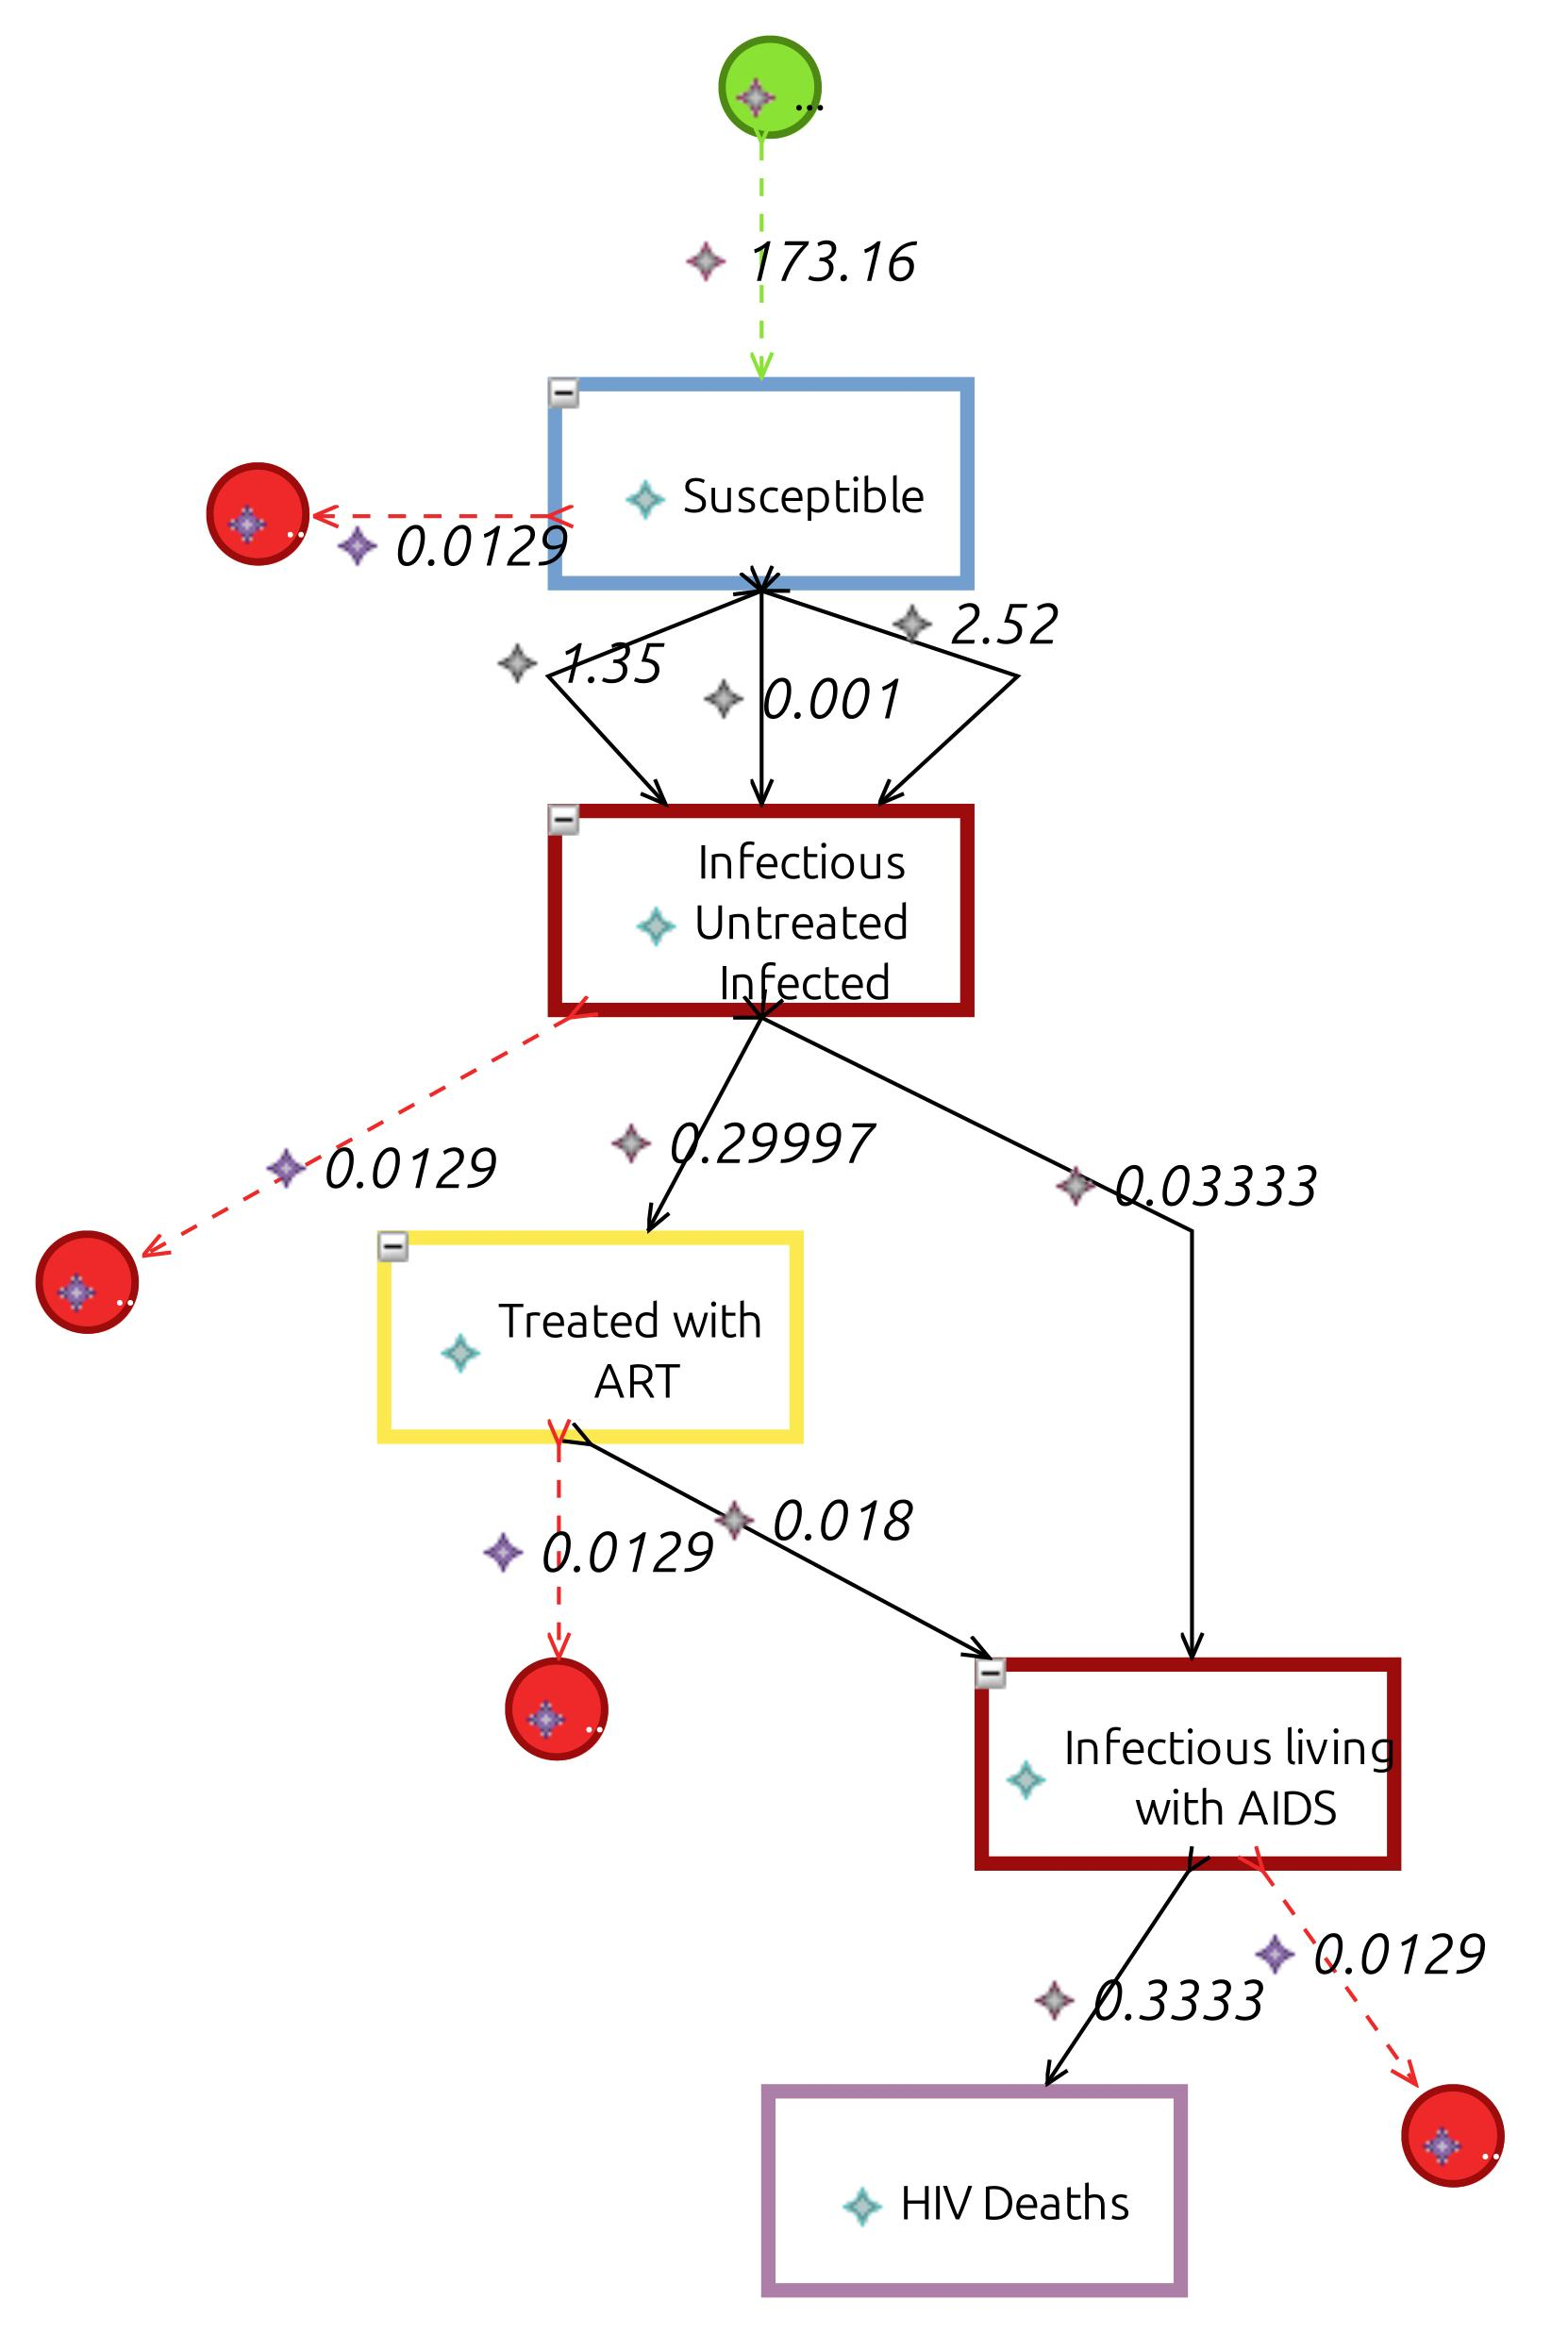
\includegraphics[width=0.5\textwidth]{Figures/HIV_Women.jpg}
    \caption{Graphical representation of the HIV-SEIR model in EpiMDE for the women demographic subgroup. Separate stratified diagrams exist for heterosexual men and homosexual men subgroups, maintaining the same compartmental structure.}
    \label{fig:hiv_model}
\end{figure}



\subsubsection{Simulation Automation}

Differential equations describing compartmental dynamics were automatically generated from the graphical representation, providing a robust mathematical foundation for simulations.

A Python script was developed to automate the simulation input process, enhancing usability by streamlining the following steps:
\begin{enumerate}
    \item Reading automatically generated .txt files containing differential equations.
    \item Guiding the user to select compartments for simulation.
    \item Collecting initial population sizes for each compartment.
    \item Specifying the simulation duration.
    \item Generating simulation outputs in .csv format, compatible with Excel or Google Sheets for further analysis.
\end{enumerate}
The results of the simulation were identical to those presented in the original publication showing the correctness and completeness of our model.



\subsubsection{LLM-Based Automated Generation Results}



To evaluate the LLM pipeline's capability to automatically generate the HIV model from textual specifications, we provided structured plain-text descriptions of the model's compartments, parameters, flows, and stratification structure to both GPT-4o and Gemini 2.5 Pro. The specification contained 66 total elements including compartments with behavioral stratification (sexual behavior groups), contact-based and rate-based flows, demographic sources and sinks, and stratum-specific transmission parameters.

\begin{table}[htbp]
\centering
\caption{LLM Performance for HIV Model Generation}
\label{tab:hiv_llm_performance}
\begin{tabular}{lccc}
\hline
\textbf{LLM Model} & \textbf{Precision} & \textbf{Recall} & \textbf{F1 Score} \\
\hline
GPT-4o & 86.4\% & 86.4\% & 0.864 \\
Gemini 2.5 Pro & 83.3\% & 100\% & 0.909 \\
\hline
\end{tabular}
\end{table}

\textbf{GPT-4o Performance:} The pipeline achieved balanced performance with Precision = 86.4\%, Recall = 86.4\%, and F1 = 0.864. All core structural elements were correctly generated: compartments with proper stratification references, the Group-Product structure for behavioral stratification, all 23 parameters with Unicode Greek letters and subscripts preserved, and birth/death sources with correct stratum assignments. The 9 false negatives and 9 false positives were primarily attributable to indexing errors in flow references—the LLM occasionally generated incorrect 0-based indices for \texttt{target} and \texttt{rateParameter} attributes. Critically, the structural integrity of the model was preserved; only specific numerical index values in flow references were incorrect. The generated simulation script (Stage 3) executed successfully, producing time-series plots for all stratified compartments with consistent variable naming and no runtime errors.

\textbf{Gemini 2.5 Pro Performance:} This model achieved perfect recall (100\%) but lower precision (83.3\%), yielding F1 = 0.909. Unlike GPT-4o, Gemini generated all 66 required elements with no omissions, demonstrating superior completeness. The 11 false positives consisted of indexing errors similar to GPT-4o and placeholder value hallucinations where the model inserted \texttt{rate="0.0"} attributes in parametric flows despite user input specifying only parameter references. This represents the LLM filling perceived specification gaps based on external modeling knowledge rather than strict input adherence. The simulation script generation succeeded with semantically organized code that grouped compartments by population, improving human readability.

\textbf{Key Findings:} Both models successfully captured the HIV model's core challenge—behavioral stratification with heterogeneous contact patterns—though with different error profiles. GPT-4o balanced precision and recall through conservative generation, while Gemini optimized for completeness at the cost of over-generation. The indexing errors shared by both models highlight a fundamental LLM limitation in tracking numerical references across many elements, suggesting the need for post-processing validation or intermediate index mapping steps. The perfect simulation script execution by both models validates the two-phase skeleton approach for code generation.

\subsection{Case Study 2: COVID-19}
\label{sec:casestudy:covid}

In our second case study, we demonstrate the use of the basic and extensible metamodels and of the modeling platform in the context of COVID-19 modeling. More specifically, we took the work of Tuite et al.~\cite{TuiteE497} on the mathematical modeling of COVID-19 transmission and mitigation strategies and we replicated the presented model using the proposed metamodel and modeling platform. We show how we can reach the same simulation results with a much reduced cognitive load, and a more concise and easier to understand model.

\subsubsection{Original model}

Figure \ref{fig:tuite1} displays the original figure from the article, Model structure of COVID-19 transmission\cite[Figure~1]{TuiteE497}. Further information in the article notes that this model is stratified along sixteen age groups as well as presence and absence of comorbidity, which will be used in equations but are absent in the graphical notation. The stratifications used by the researchers are a consequence of their available data. The population age data uses 20 intervals of 5 years and one for 100 years old or older. The contact mixing data uses 14 intervals of 5 years and one for 70 or older.

It is important to note that important information about the model was not possible to be extracted just from the manuscript, but part of it was extracted by further investigating the accompanying source code repository. This further emphasizes the need to gather all model elements under a single location to improve communication and reproducibility.

\begin{figure}[t]
    \centering
    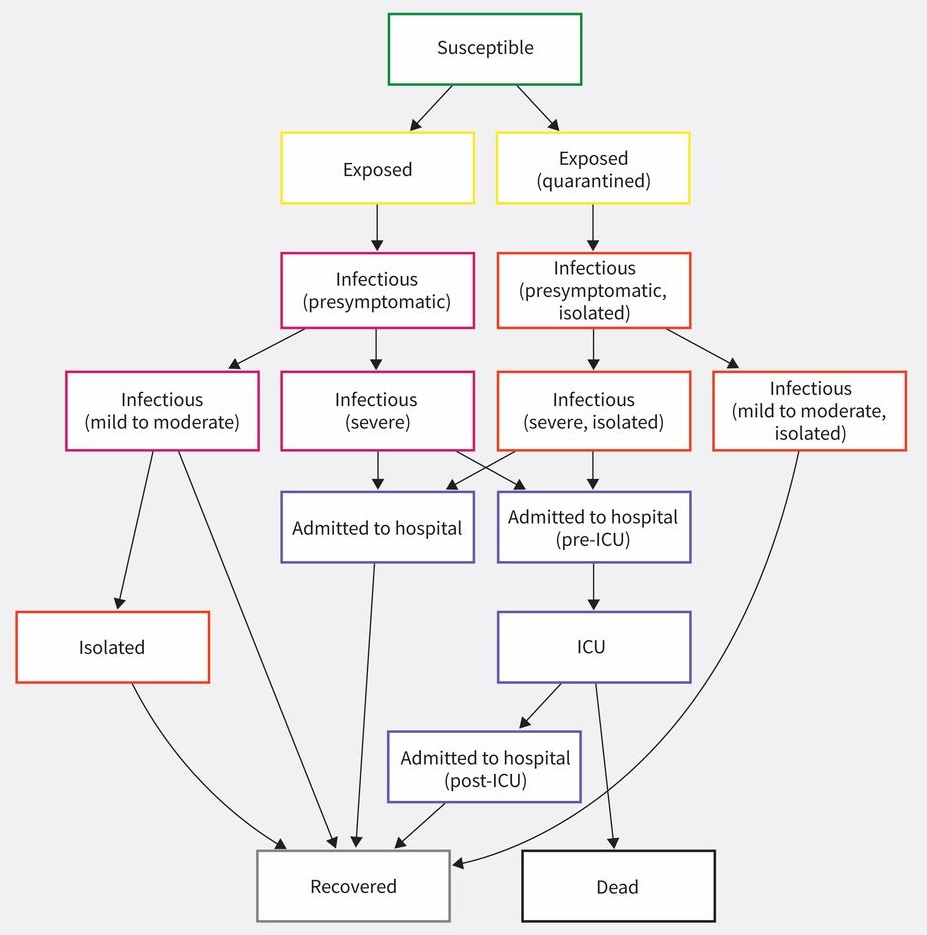
\includegraphics[width=\linewidth]{Figures/tuite1.jpg}
    \caption{Original COVID-19 Model Representation~\cite{TuiteE497}}
    \label{fig:tuite1}
\end{figure}



\subsubsection{Translated model}

In order to represent the disease model in our platform, present two approaches: using the basic metamodel (EpiMDE) and the extensible metamodel. As it can be seen in Figure~\ref{fig:covid_model}, the generated EpiMDE model is almost identical to the original model (Figure~\ref{fig:tuite1}).

\begin{figure}[htbp]
    \centering
    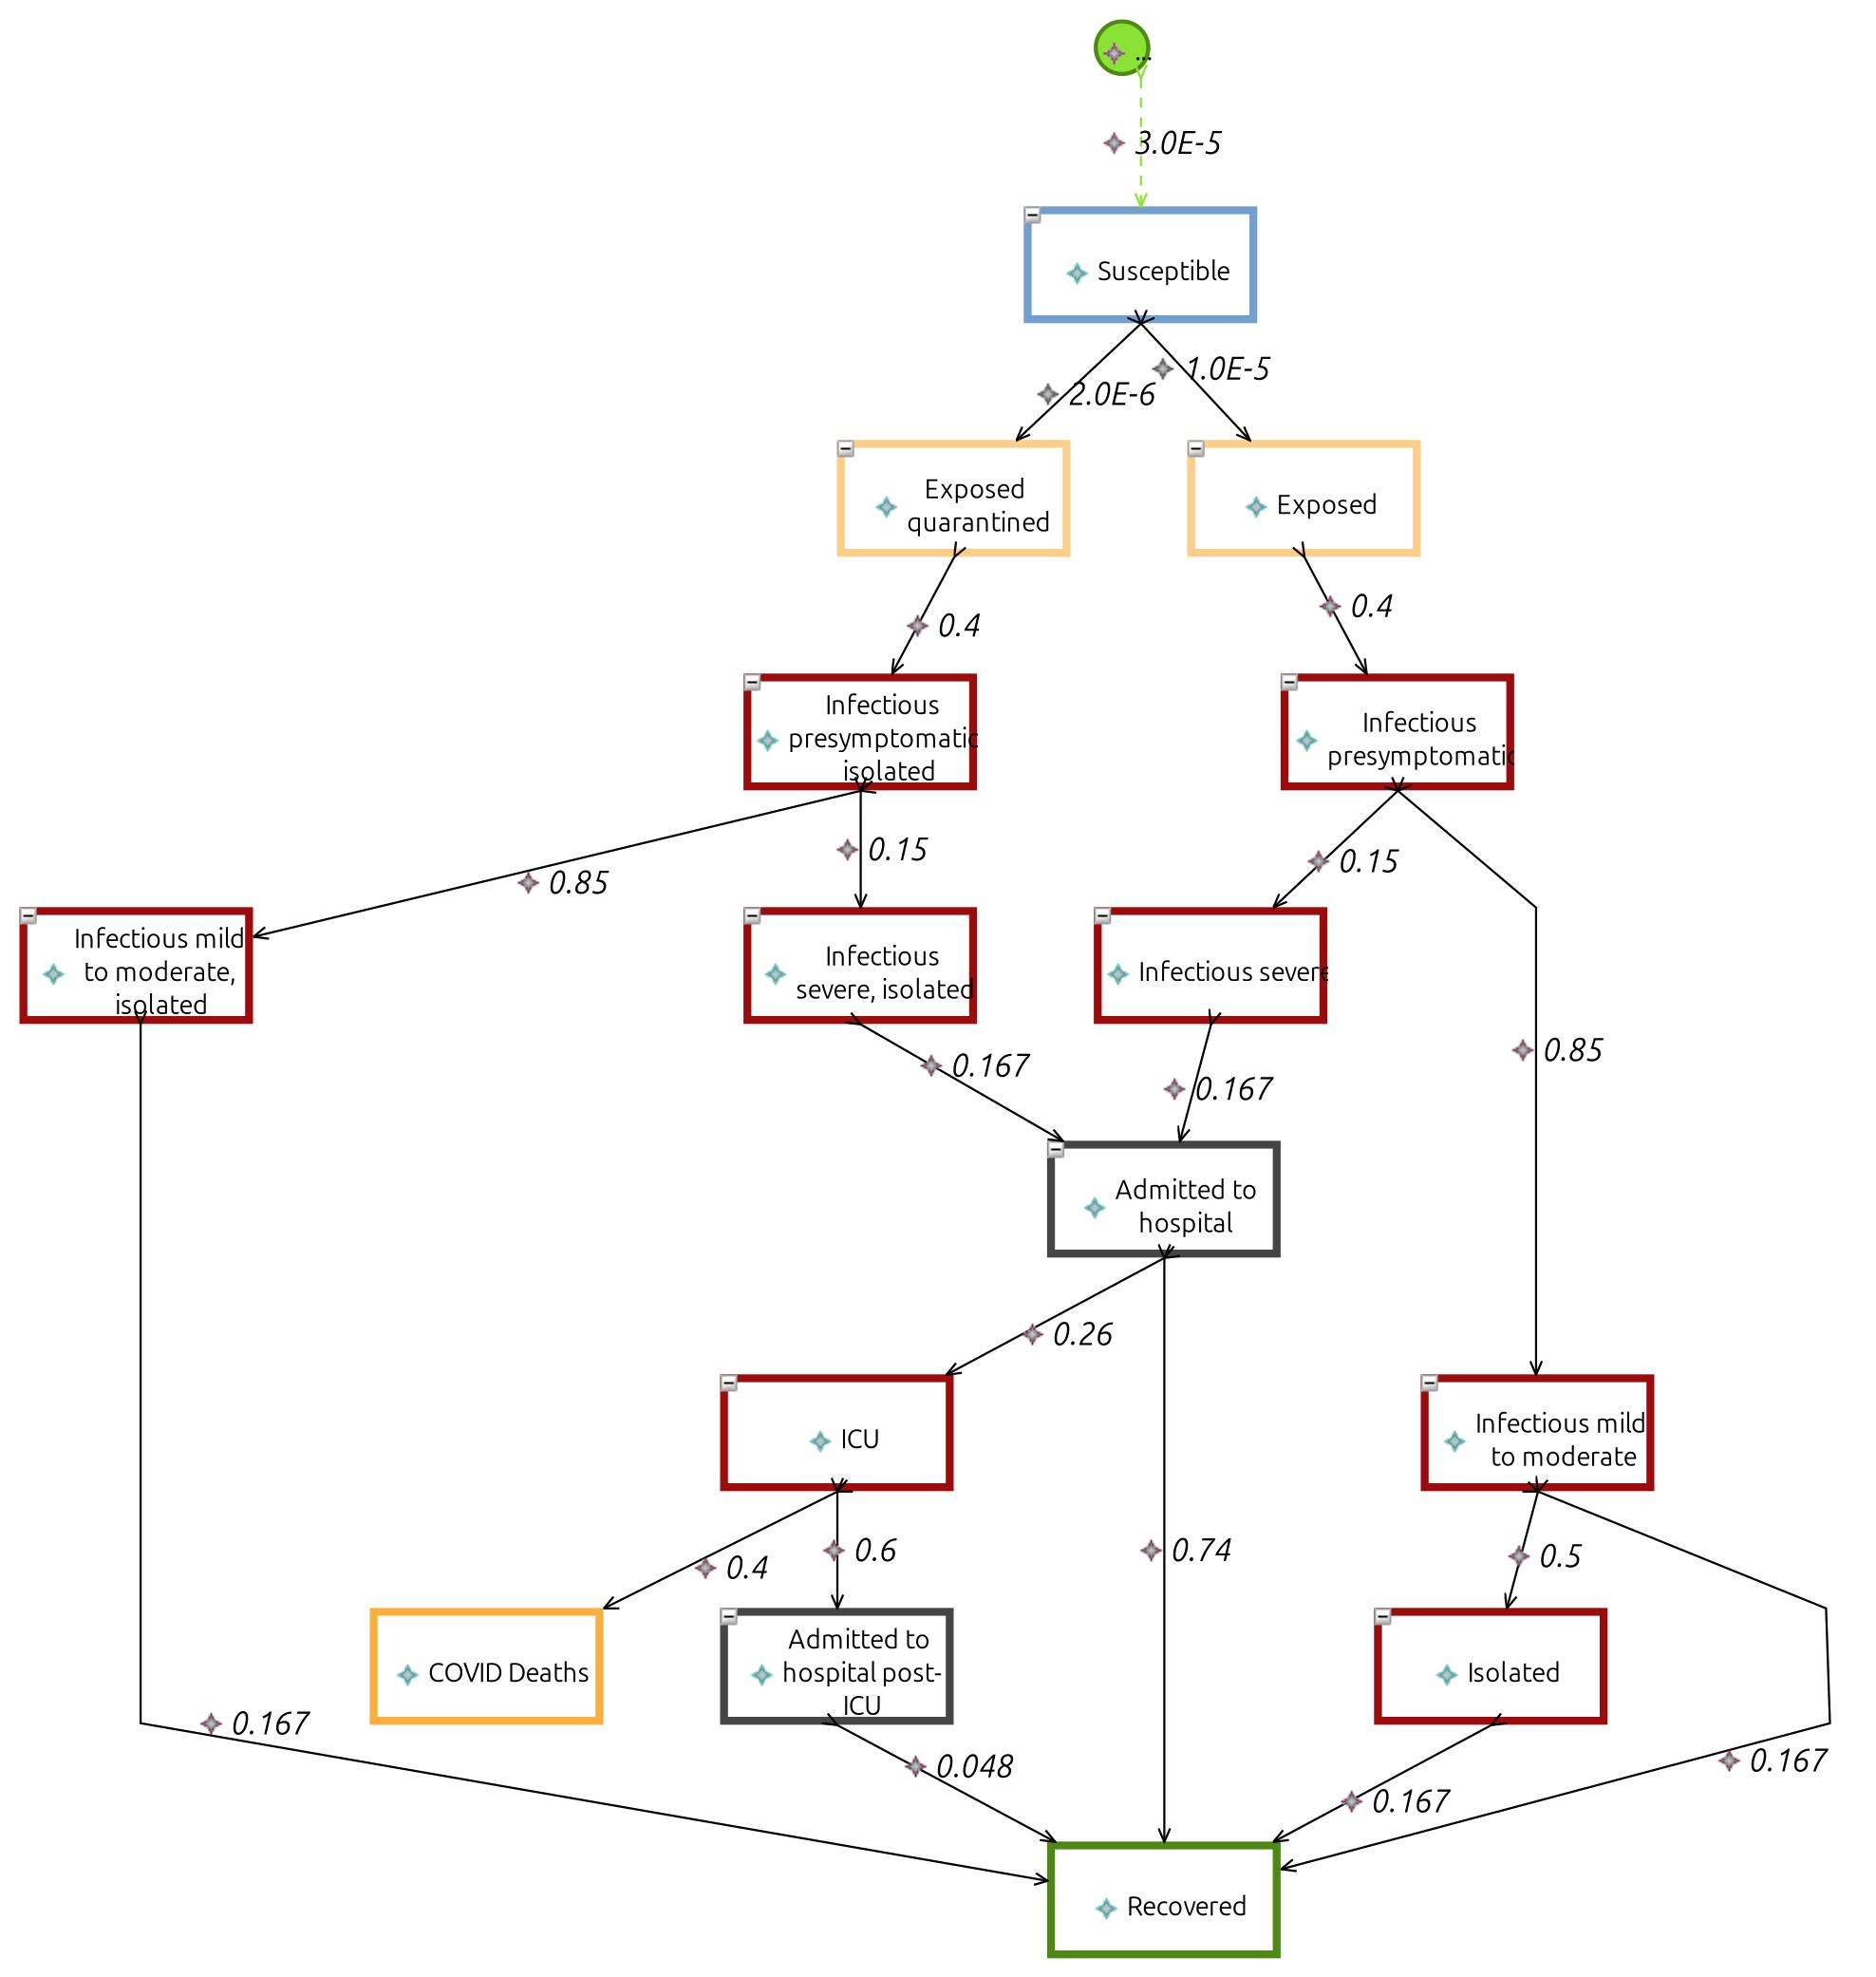
\includegraphics[width=0.8\textwidth]{Figures/Covid.jpg}
    \caption{Graphical representation of the COVID-19 SEIR model in EpiMDE Lite.}
    \label{fig:covid_model}
\end{figure}

While the basic modeling approach with EpiMDE is good for quickly replicating the original work, the resulting model suffers from the shortcomings of the original model, i.e., reduced replicability and verbosity, in terms of number of compartments and flows. In addition, certain parameters of the original model, such as age groups, could not be easily ported in the EpiMDE model. To this end, we also explored the capabilities of the extensible metamodel and we used groups and products, as well as complex flows, to better organize the model, through better modularity and separation of concerns, and facilitate more of its advance functionalities.

First, looking at the naming and coloring of the elements in the original diagram, we can see that orange refers to isolated, while purple refers to not isolated. Susceptible, exposed, hospitalized and recovered are also color coded. We begin by creating a group to place our elements into, then place unit compartments for S, R and Dead. E and I share commonalities, specifically, they are both stratified along isolation status. We will create a product to hold two groups: isolation and E-I. The isolation group simply has a isolated and non-isolated unit compartments. E-I has two groups, E and I, which have their purple and orange compartments from the original figure, so E is a compartment but I is a group containing presymptomatic, mild and severe.

%The researchers responsible for the studied model made the decision not to include "within-hospital transmission cycles"\cite{TuiteE497}. For this reason, we can leave hospitalization out of the infectious group as they will not be used as contacts for transmission. Hospitalization will be a group with units for no-icu, pre-icu, icu and post-icu. 
%Figure \ref{fig:tuite-cp1} shows the structure so far.

%\begin{figure}[H]
%    \centering
%    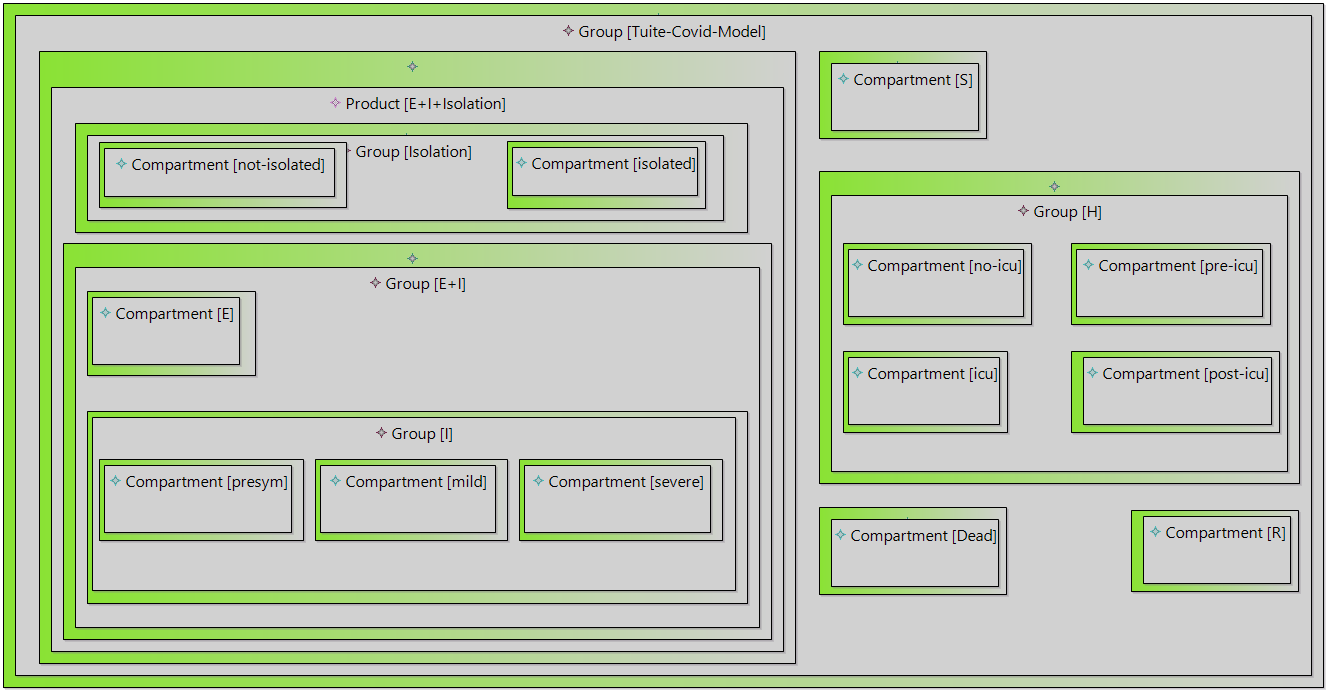
\includegraphics[width=\linewidth]{Figures/tuite-cp1.png}
%    \caption{Model Structure}
%    \label{fig:tuite-cp1}
%\end{figure}

After modeling the structural aspect of the model, it is time to model the behavioural aspect, by using flows. The original model contains 21 flows, but by using flows on composites, we can reduce this amount. As a model's size increases, applying flows to structures instead of individual components saves time and complexity. It also dissociates a composite's contents from the flows, allowing for inner structure modification without change to the flows. This is visually apparent in the resulting model, as shown in Figure \ref{fig:tuite-cp2}. There are now 11 flows instead of 21. Flows in our platform are named diamonds with named reference, which may help clarify the model. For example, the authors mention: "Testing was assumed to move individuals with nonsevere symptoms from the infectious to isolated compartments" \cite{TuiteE497}, while in our model we can simply name this flow "testing".

\begin{figure}[t]
    \centering
    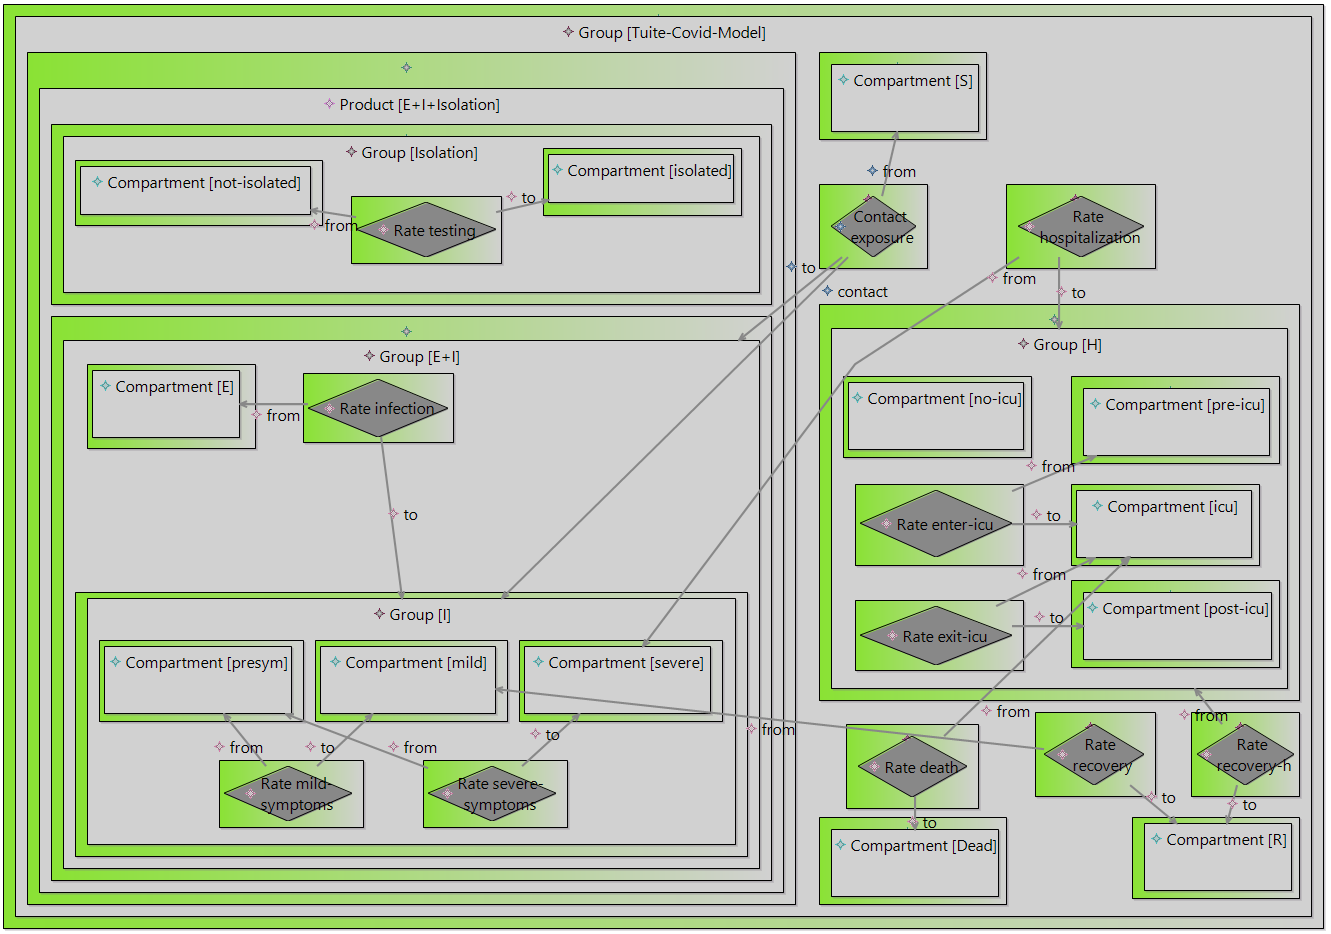
\includegraphics[width=\linewidth]{Figures/tuite-cp2.png}
    \caption{Model Structure and Flows}
    \label{fig:tuite-cp2}
\end{figure}


The final step is model stratification along age and comorbidity, which is simply done by placing the model in a product along with the age dimension and the comorbidity dimension. As seen in the original model, stratification along age and comorbidity is not represented graphically, which is not the case for EpiMDE. The result is a simple model of a product between age groups, which can be used in the larger model as a link (i.e., an expandable reference to an external model), and a comorbidity option.
%, as shown in Figure~\ref{fig:tuite-cp4}.

%\begin{figure}[H]
%    \centering
%    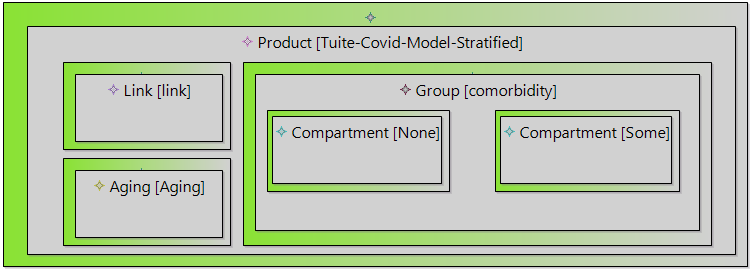
\includegraphics[width=\linewidth]{Figures/tuite-cp4.png}
%    \caption{Stratified Model}
%    \label{fig:tuite-cp4}
%\end{figure}

The Link and Aging compartments are simple metamodel extensions. Link allows us to reference compartments from other model, here we reference the top level element from the previous model. Aging allows us to provide a list of age groups as a string, in this case, for the Canadian health data, we provide ``0-4, 5-9, 10-14, 15-19, 20-24, 25-29, 30-34, 35-39, 40-44, 45-49, 50-54, 55-59, 60-64, 65-69, 70+", which generates compartments as well as rates between the consecutive age groups.

\subsubsection{Model validation}

Model validation involves comparing the expected output of a model with the actual output. The output may be thought of as the graph produced for an entire simulation, but, in practice, this may change based on simulation software. The derivative produced given a population distribution, however, is predictable.

In order to compare models, we randomly generated population distributions to compare both models' derivatives. The reference model's derivative is the expected derivative of the model being validated. In the event where the two are identical, the validation is done. In the event where the two are different, we need to refine the incorrect model and ideally identify where the differences come from. This is an aspect of the project which presents an opportunity for usability improvements.

For the context of this work, a validation script was produced which iterates over the names of our flows of this specific model and produces derivatives for both models based on an input. The original R code was transpiled to python and its equations were deconstructed in order to map the terms to names of equation. By writing a validation script which validates a projection of the model along a single equation, it is much easier to refine. Since flows in our platform are named and names are kept in the artifacts, we can easily toggle certain sets of equations by name. In the future, model validation may be further automated so that little to no programming may be involved for similar use cases, rendering this task simpler for epidemiologists.

\subsubsection{LLM-Based Automated Generation Results}

The COVID-19 model presented a more complex generation challenge than HIV, with 63 total elements including 15 compartments across multiple disease stages (exposed, infectious subtypes, hospitalization states), 23 parameters, age-based stratification, and 19 flows representing disease progression and intervention pathways. This model's larger element count and intricate flow network tested the LLM pipeline's scalability.

\begin{table}[htbp]
\centering
\caption{LLM Performance for COVID-19 Model Generation}
\label{tab:covid_llm_performance}
\begin{tabular}{lccc}
\hline
\textbf{LLM Model} & \textbf{Precision} & \textbf{Recall} & \textbf{F1 Score} \\
\hline
GPT-4o & 91.1\% & 65.1\% & 0.759 \\
Gemini 2.5 Pro & 100\% & 100\% & 1.000 \\
\hline
\end{tabular}
\end{table}

\textbf{GPT-4o Performance:} The pipeline achieved high precision (91.1\%) but significantly lower recall (65.1\%), yielding F1 = 0.759. While compartments, parameters, groups, and products were correctly generated, 22 of the 19 specified flows were either completely absent or generated with incorrect structure. The user input clearly listed all flow transitions, but these did not materialize in the final XML with proper \texttt{<outgoingFlows>} elements. This failure mode differs fundamentally from the HIV model's indexing errors and suggests two contributing factors: context window pressure from the substantially larger specification approaching GPT-4o's effective context limits, and potential prompt ambiguity in translating complex flow networks into XML. The 4 false positives represented attribute hallucination where the model generated \texttt{multiplier} attributes within \texttt{<stratumSpecificRates>} for age-dependent transmission rates—conceptually reasonable but not part of the metamodel specification. Despite XML generation challenges, the Stage 3 simulation script executed successfully using validated ODE equations, producing correct time-series plots for all age-stratified compartments.

\textbf{Gemini 2.5 Pro Performance:} In stark contrast to GPT-4o, Gemini achieved perfect generation with Precision = 100\%, Recall = 100\%, F1 = 1.000. All 63 elements were correctly generated with no hallucinations and no omissions. Critically, all 19 flows appeared with proper structure, correct \texttt{xsi:type} classification (RateFlow vs. ContactFlow), accurate \texttt{target} references, and appropriate parameter linkages. The flow omission pattern that plagued GPT-4o did not occur, suggesting the failure was not inherent to task complexity but specific to GPT-4o's context management or instruction-following capabilities for this prompt structure. The simulation script generation succeeded with compact, semantically organized code that logically grouped compartments and improved human readability while maintaining 100\% execution correctness.

\textbf{Key Findings:} The dramatic performance divergence between GPT-4o and Gemini reveals that COVID-19 model generation is a context-intensive task requiring state-of-the-art LLM capabilities. GPT-4o's systematic flow omissions indicate it reached capacity limits handling the specification's size and complexity, while Gemini's perfect generation demonstrates that frontier models possess sufficient capacity for complex epidemiological models. This has practical implications: as models grow in complexity (more compartments, deeper stratification, intricate interventions), access to cutting-edge LLMs transitions from optional to necessary. The perfect simulation generation by both models (despite XML differences) again validates the robustness of the two-phase skeleton approach, which successfully isolated Stage 3 from Stage 1-2 errors by operating on independently validated ODE equations.



\subsection{Case Study 3: Illustrating Support for Rapid Prototyping}
\label{sec:casestudy:prototyping}
% \subsection{Introduction and Motiv<ating Example}
% \label{subsec:carol-example-introduction}


EpiMDE is designed to support workflow extensions implemented as separate layers on top of the core platform. It exposes the metamodel and model repository through an EMF based API, enabling external analyses (e.g., clustering, differencing, logical consistency checks) to be integrated without modifying the platform itself. In our third case study, we examine how well EpiMDE supports epidemiological workflows, by developing an illustrative example. 
Specifically, we use a rapid prototyping scenario~\cite{fiyouzisabah2024towards} to probe whether the platform provides sufficient expressiveness and extensibility to support the construction of workflow-specific tooling on top of EpiMDE.
% Specifically, we probed how well the platform can be used to build a tool for rapid prototyping of epidemiological models, in a context that arises when a new disease is discovered. 
We studied the research question: 
\textit{What challenges and opportunities arise when applying a purpose-built modeling infrastructure to the development of domain-specific modeling workflows?} 
The lessons learned reveal both the platform’s strengths and its friction points.

We assume a persona named ``Carol'' working under the pressure of a health crisis (like the COVID-19 pandemic) to quickly create and validate an epidemiological model. 
Carol hopes to rapidly prototype a new model by reusing previously developed, tested, and validated model components to accelerate her work. 
So, she wants to identify and select useful modeling elements and assemble them into a partially completed prototype, avoiding redundant re‐implementation efforts. 
She hopes that, using this prototype model as a base, she can focus on her study's unique aspects and design and integrate new features. 
All models and generated artifacts from our scenario are included in our replication package published on Zenodo~\cite{zenodo_17806440}.

We assume that Carol starts with a corpus made up of the three previously developed compartmental models shown in Figure~\ref{fig:prototype_submodels}. 
Each one contains elements that may be relevant and useful for her own study. 
For instance, the model $m_1$ in Figure~\ref{fig:prototype_m1} includes exposed and vaccinated groups.
The model $m_2$ in Figure~\ref{fig:prototype_m2} adds more details about disease spread by breaking down the infectious population into asymptomatic, mildly symptomatic, and severely symptomatic compartments. 
Finally, the model $m_3$ in Figure~\ref{fig:prototype_m3} contains the hospitalization status of individuals, allowing to better model the load to the healthcare system.
Typically, Carol would have to manually search through the corpus of existing models, identify which parts are relevant, extract them, and then integrate them into her own model.
This is time-consuming and error-prone. 
Using the EpiMDE platform, we can simplify this process by creating an interactive layer that guides users like Carol through the steps for reusing previous work. 
Carol only needs to provide a repository of existing models. 
The tool then follows the workflow explained later (see Subsection~\ref{sec:prototyping_workflow}) to analyze these models and identify potentially relevant components. 
Finally, Carol can select the parts she wants to reuse, and the tool will automatically generate a prototype model that includes the selected items. 
She can then use this as a partially completed prototype on which to base the rest of her modeling efforts. 

\begin{figure}[t]
\centering
\begin{subfigure}[b]{0.40\textwidth}
  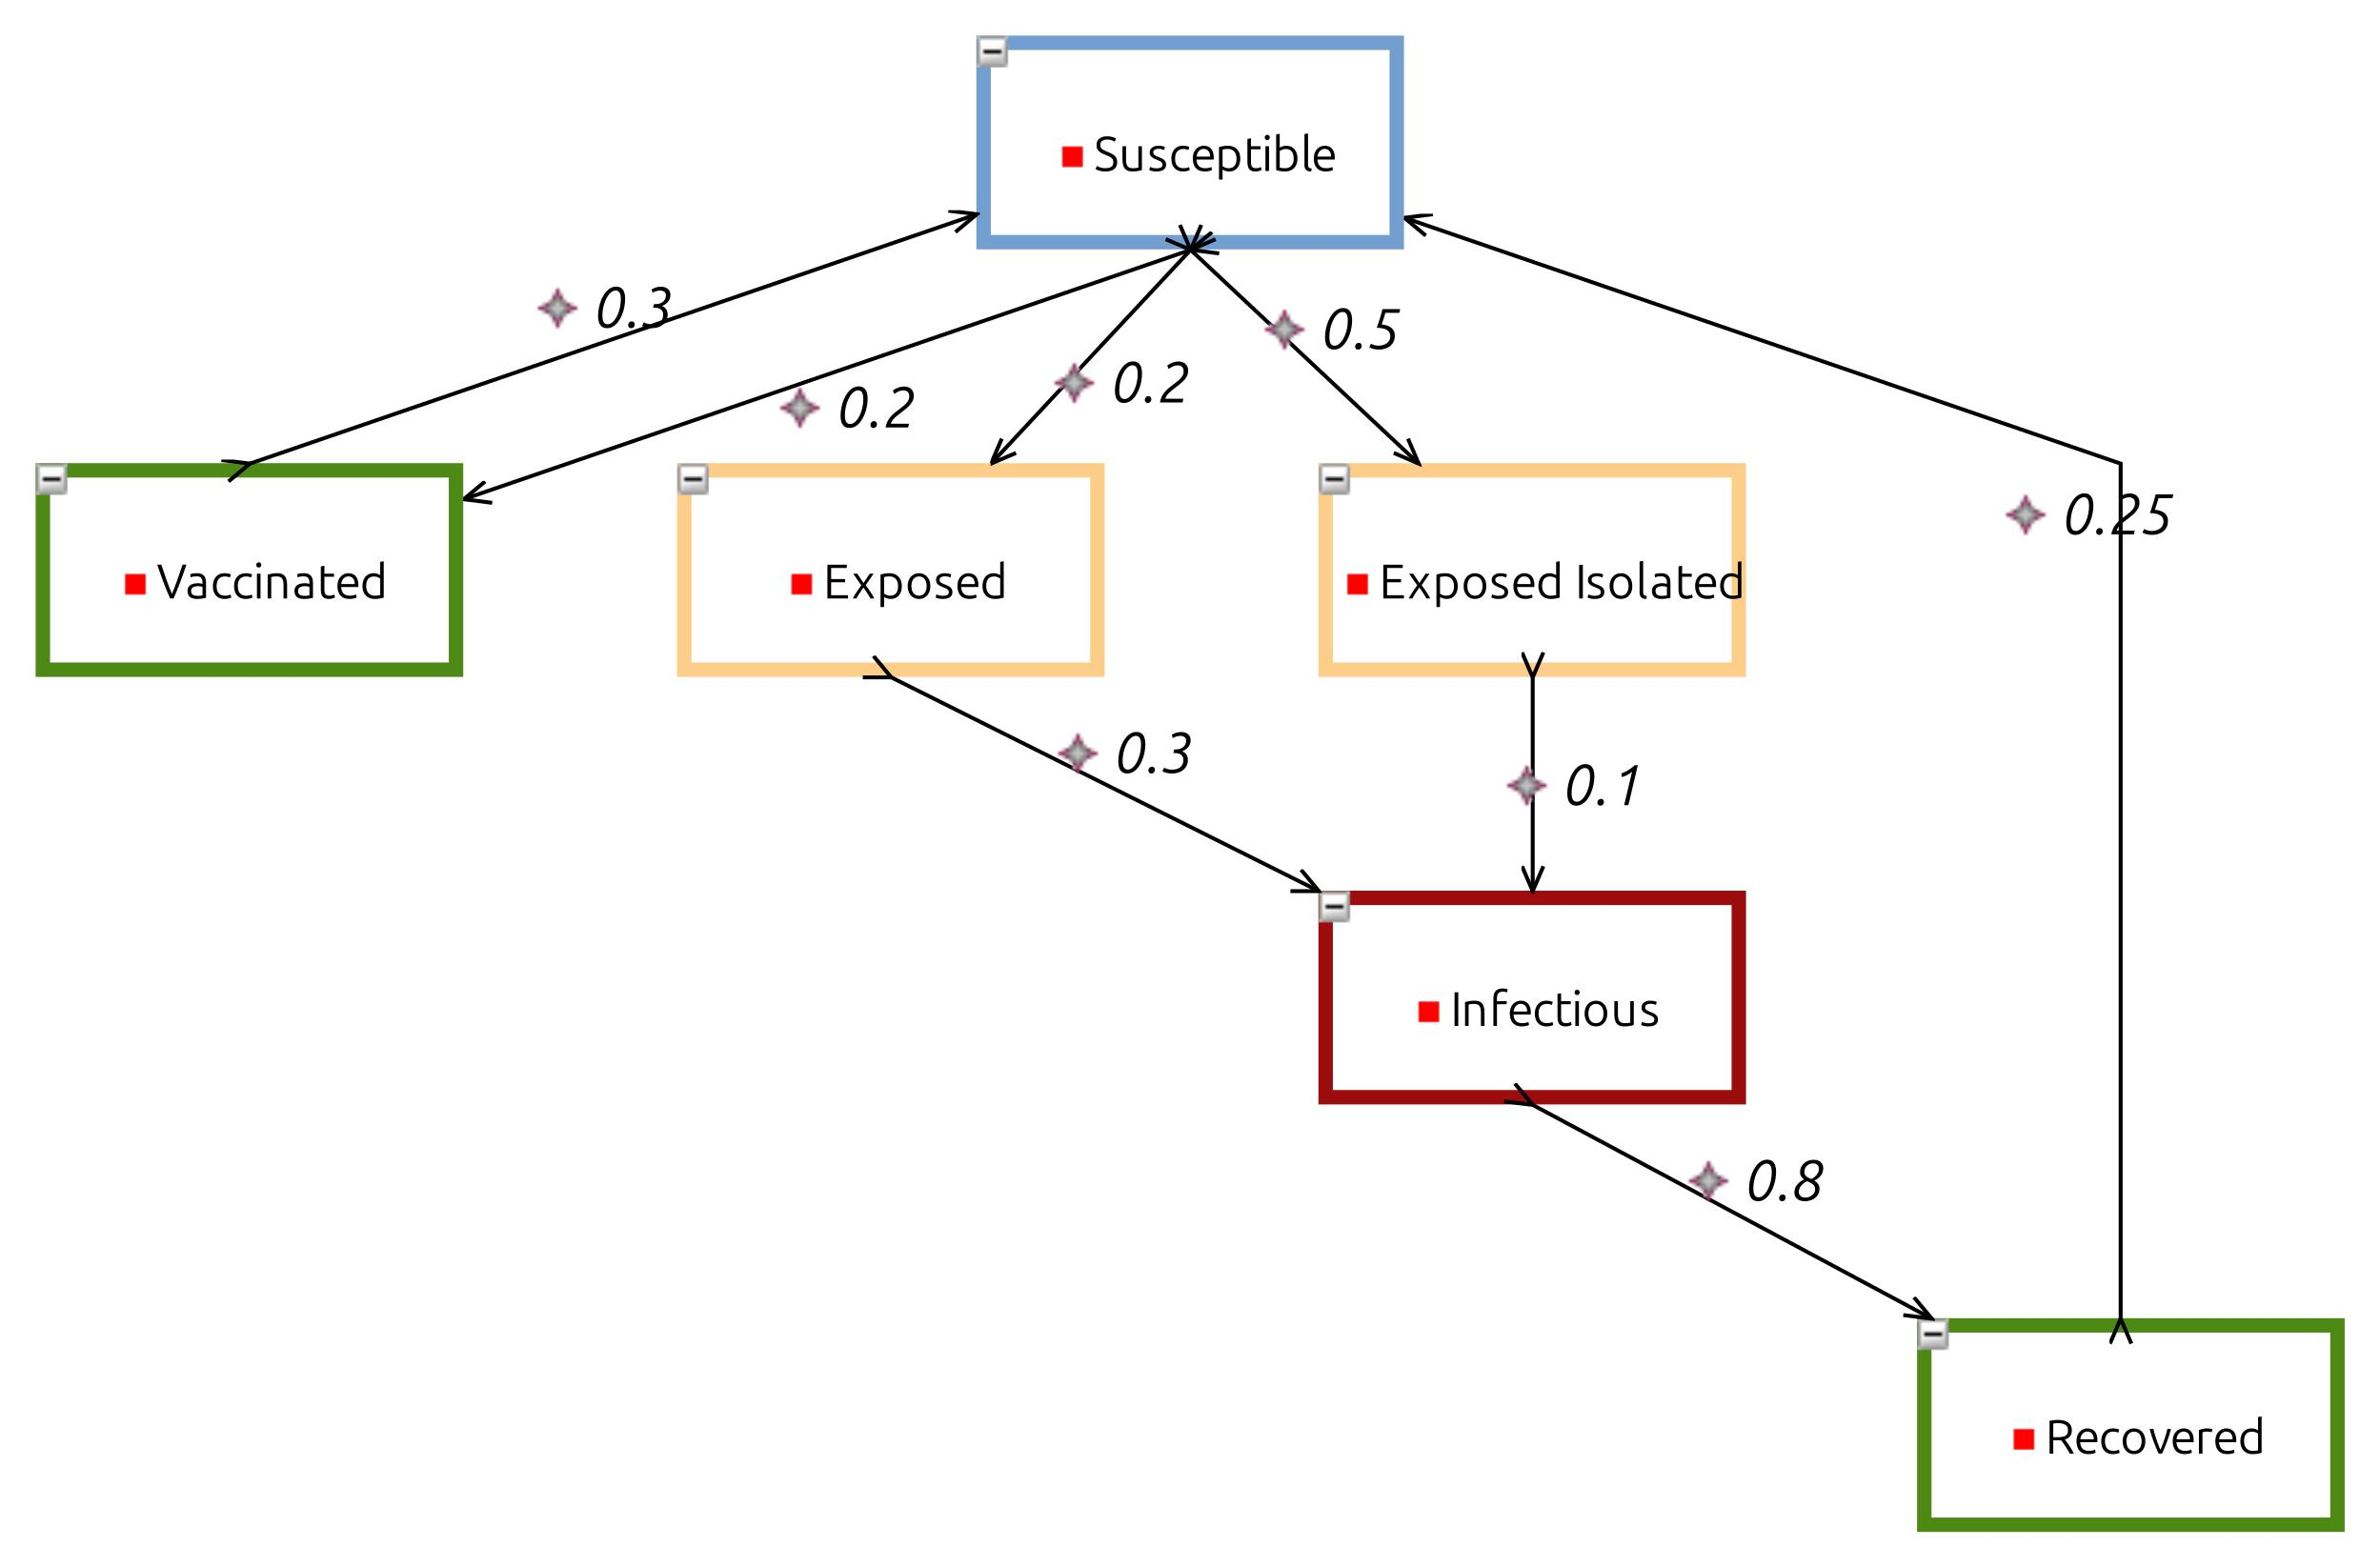
\includegraphics[width=\textwidth]{Figures/paper1.jpg}
  \caption{$m_1$}
  \label{fig:prototype_m1}
\end{subfigure}
\begin{subfigure}[b]{0.40\textwidth}
  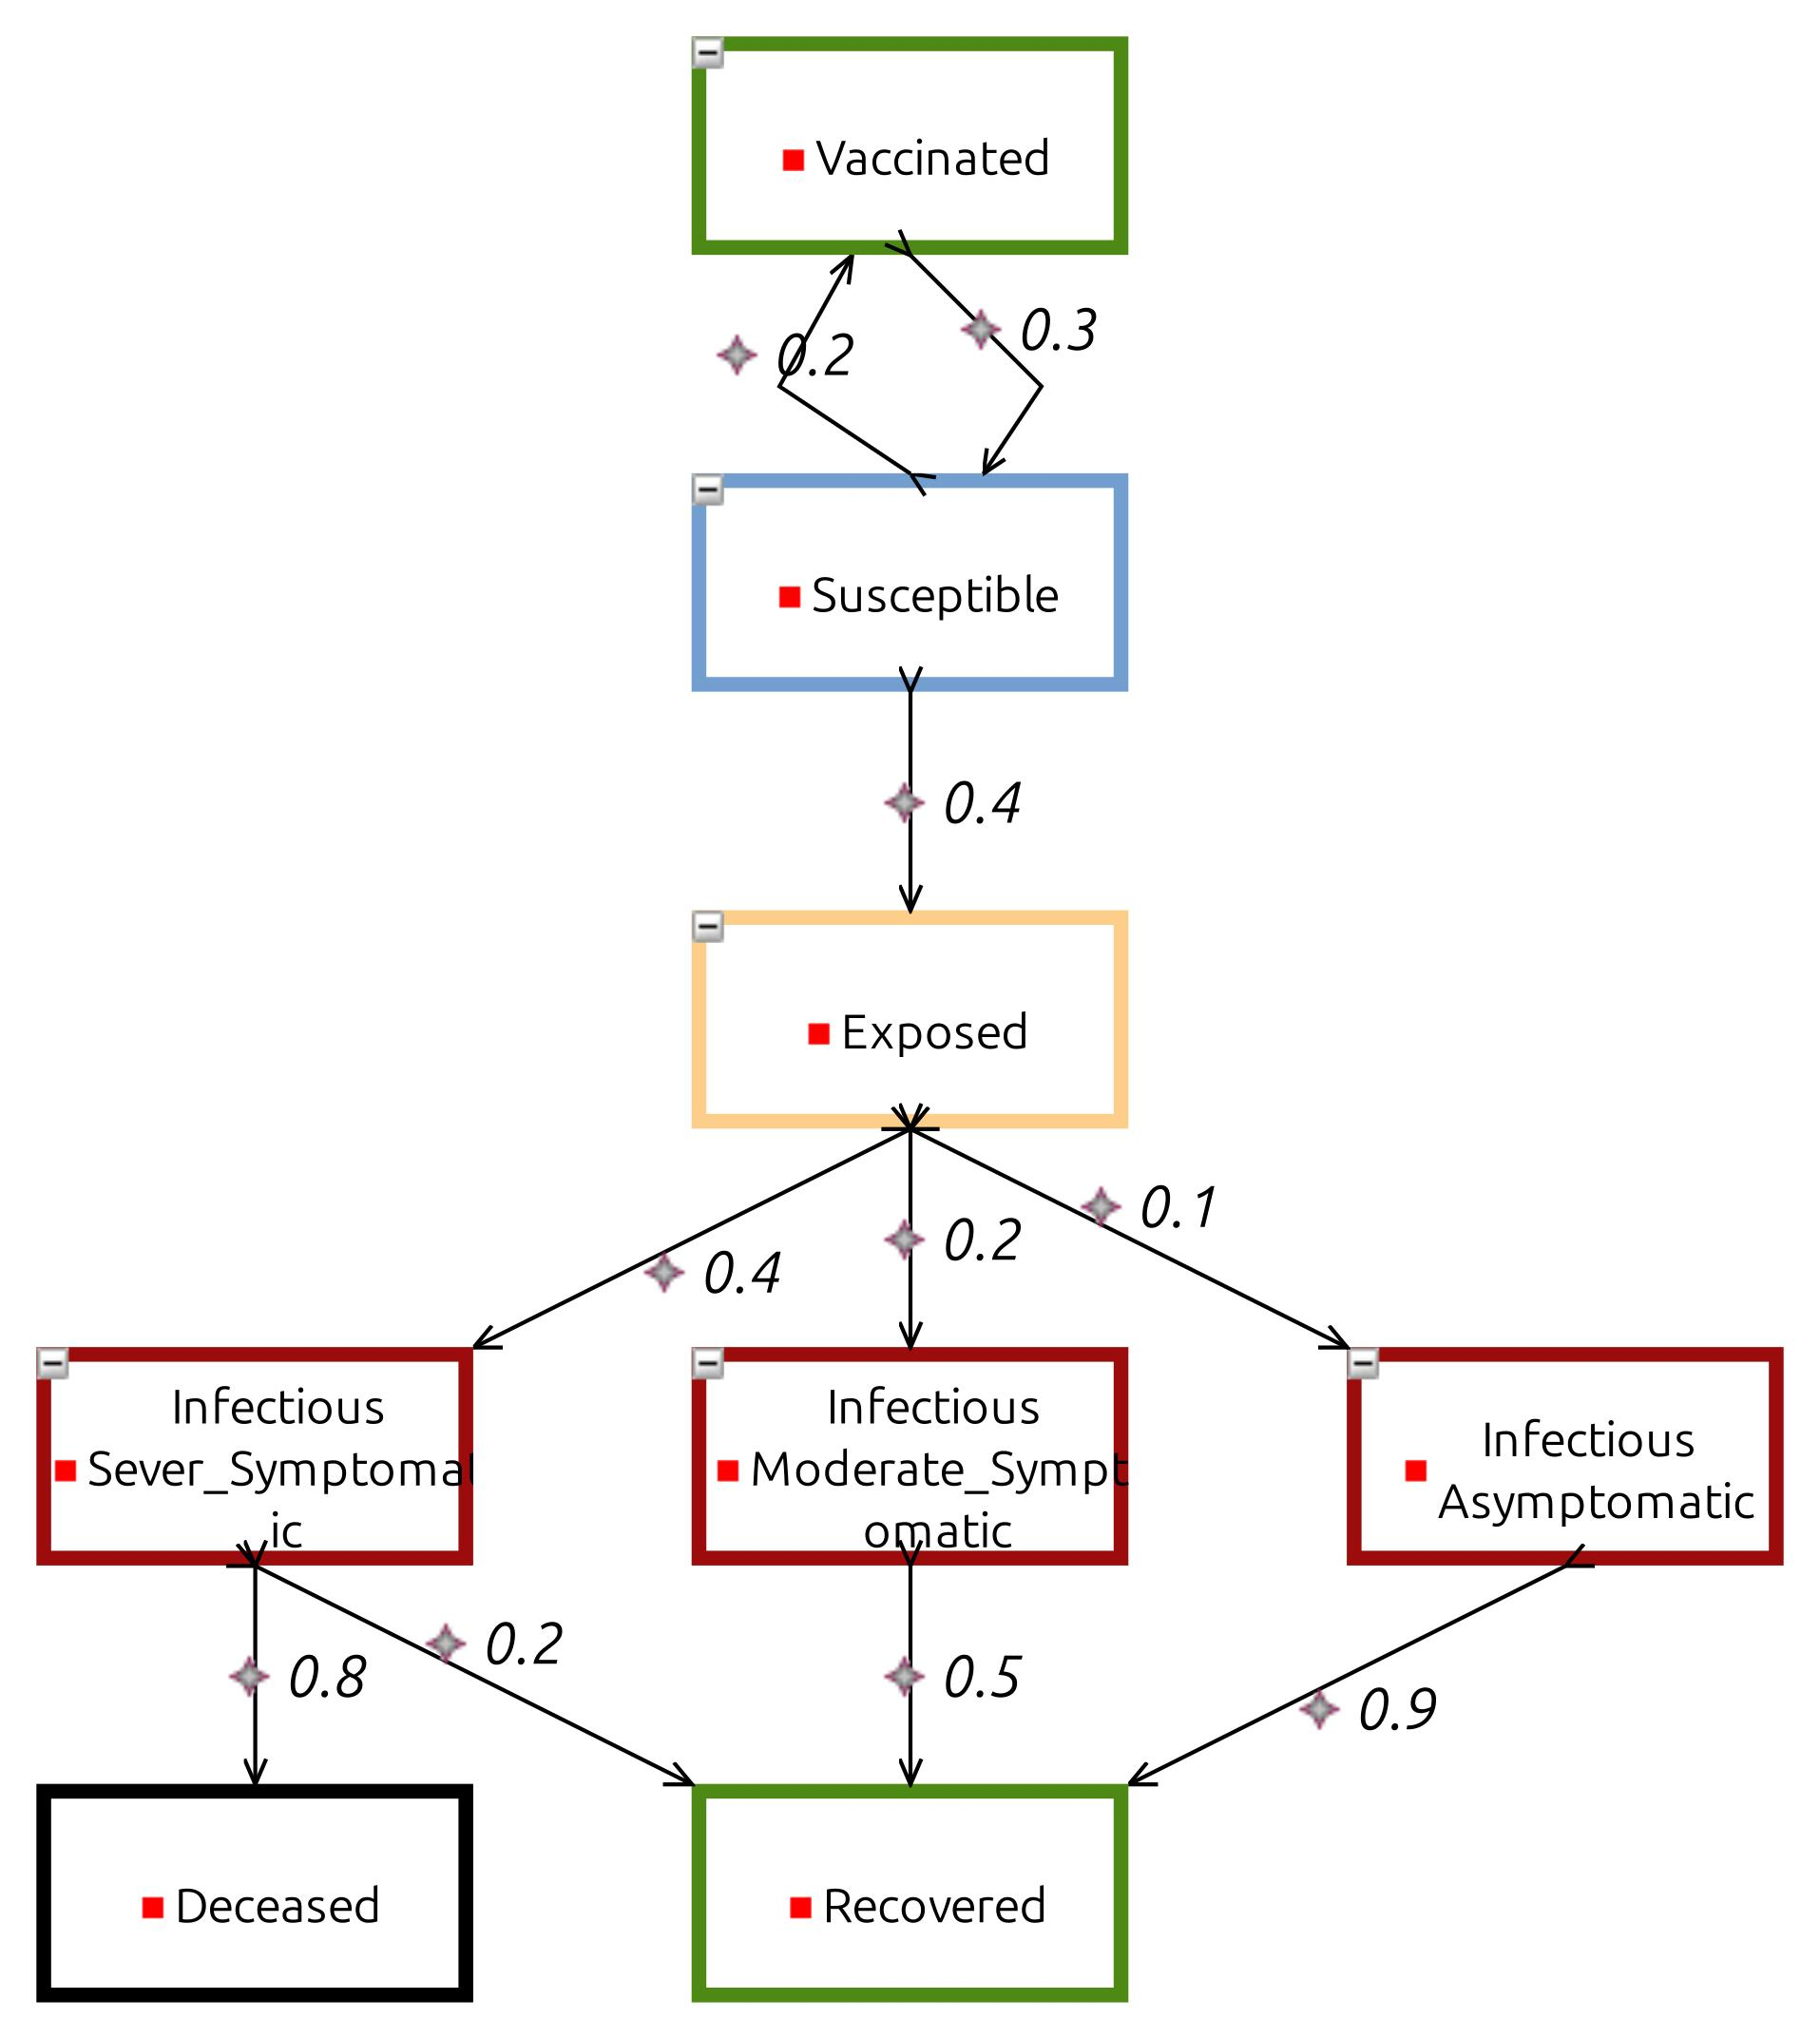
\includegraphics[width=\textwidth]{Figures/paper2.jpg}
  \caption{$m_2$}
  \label{fig:prototype_m2}
\end{subfigure}
\begin{subfigure}[b]{0.40\textwidth}
  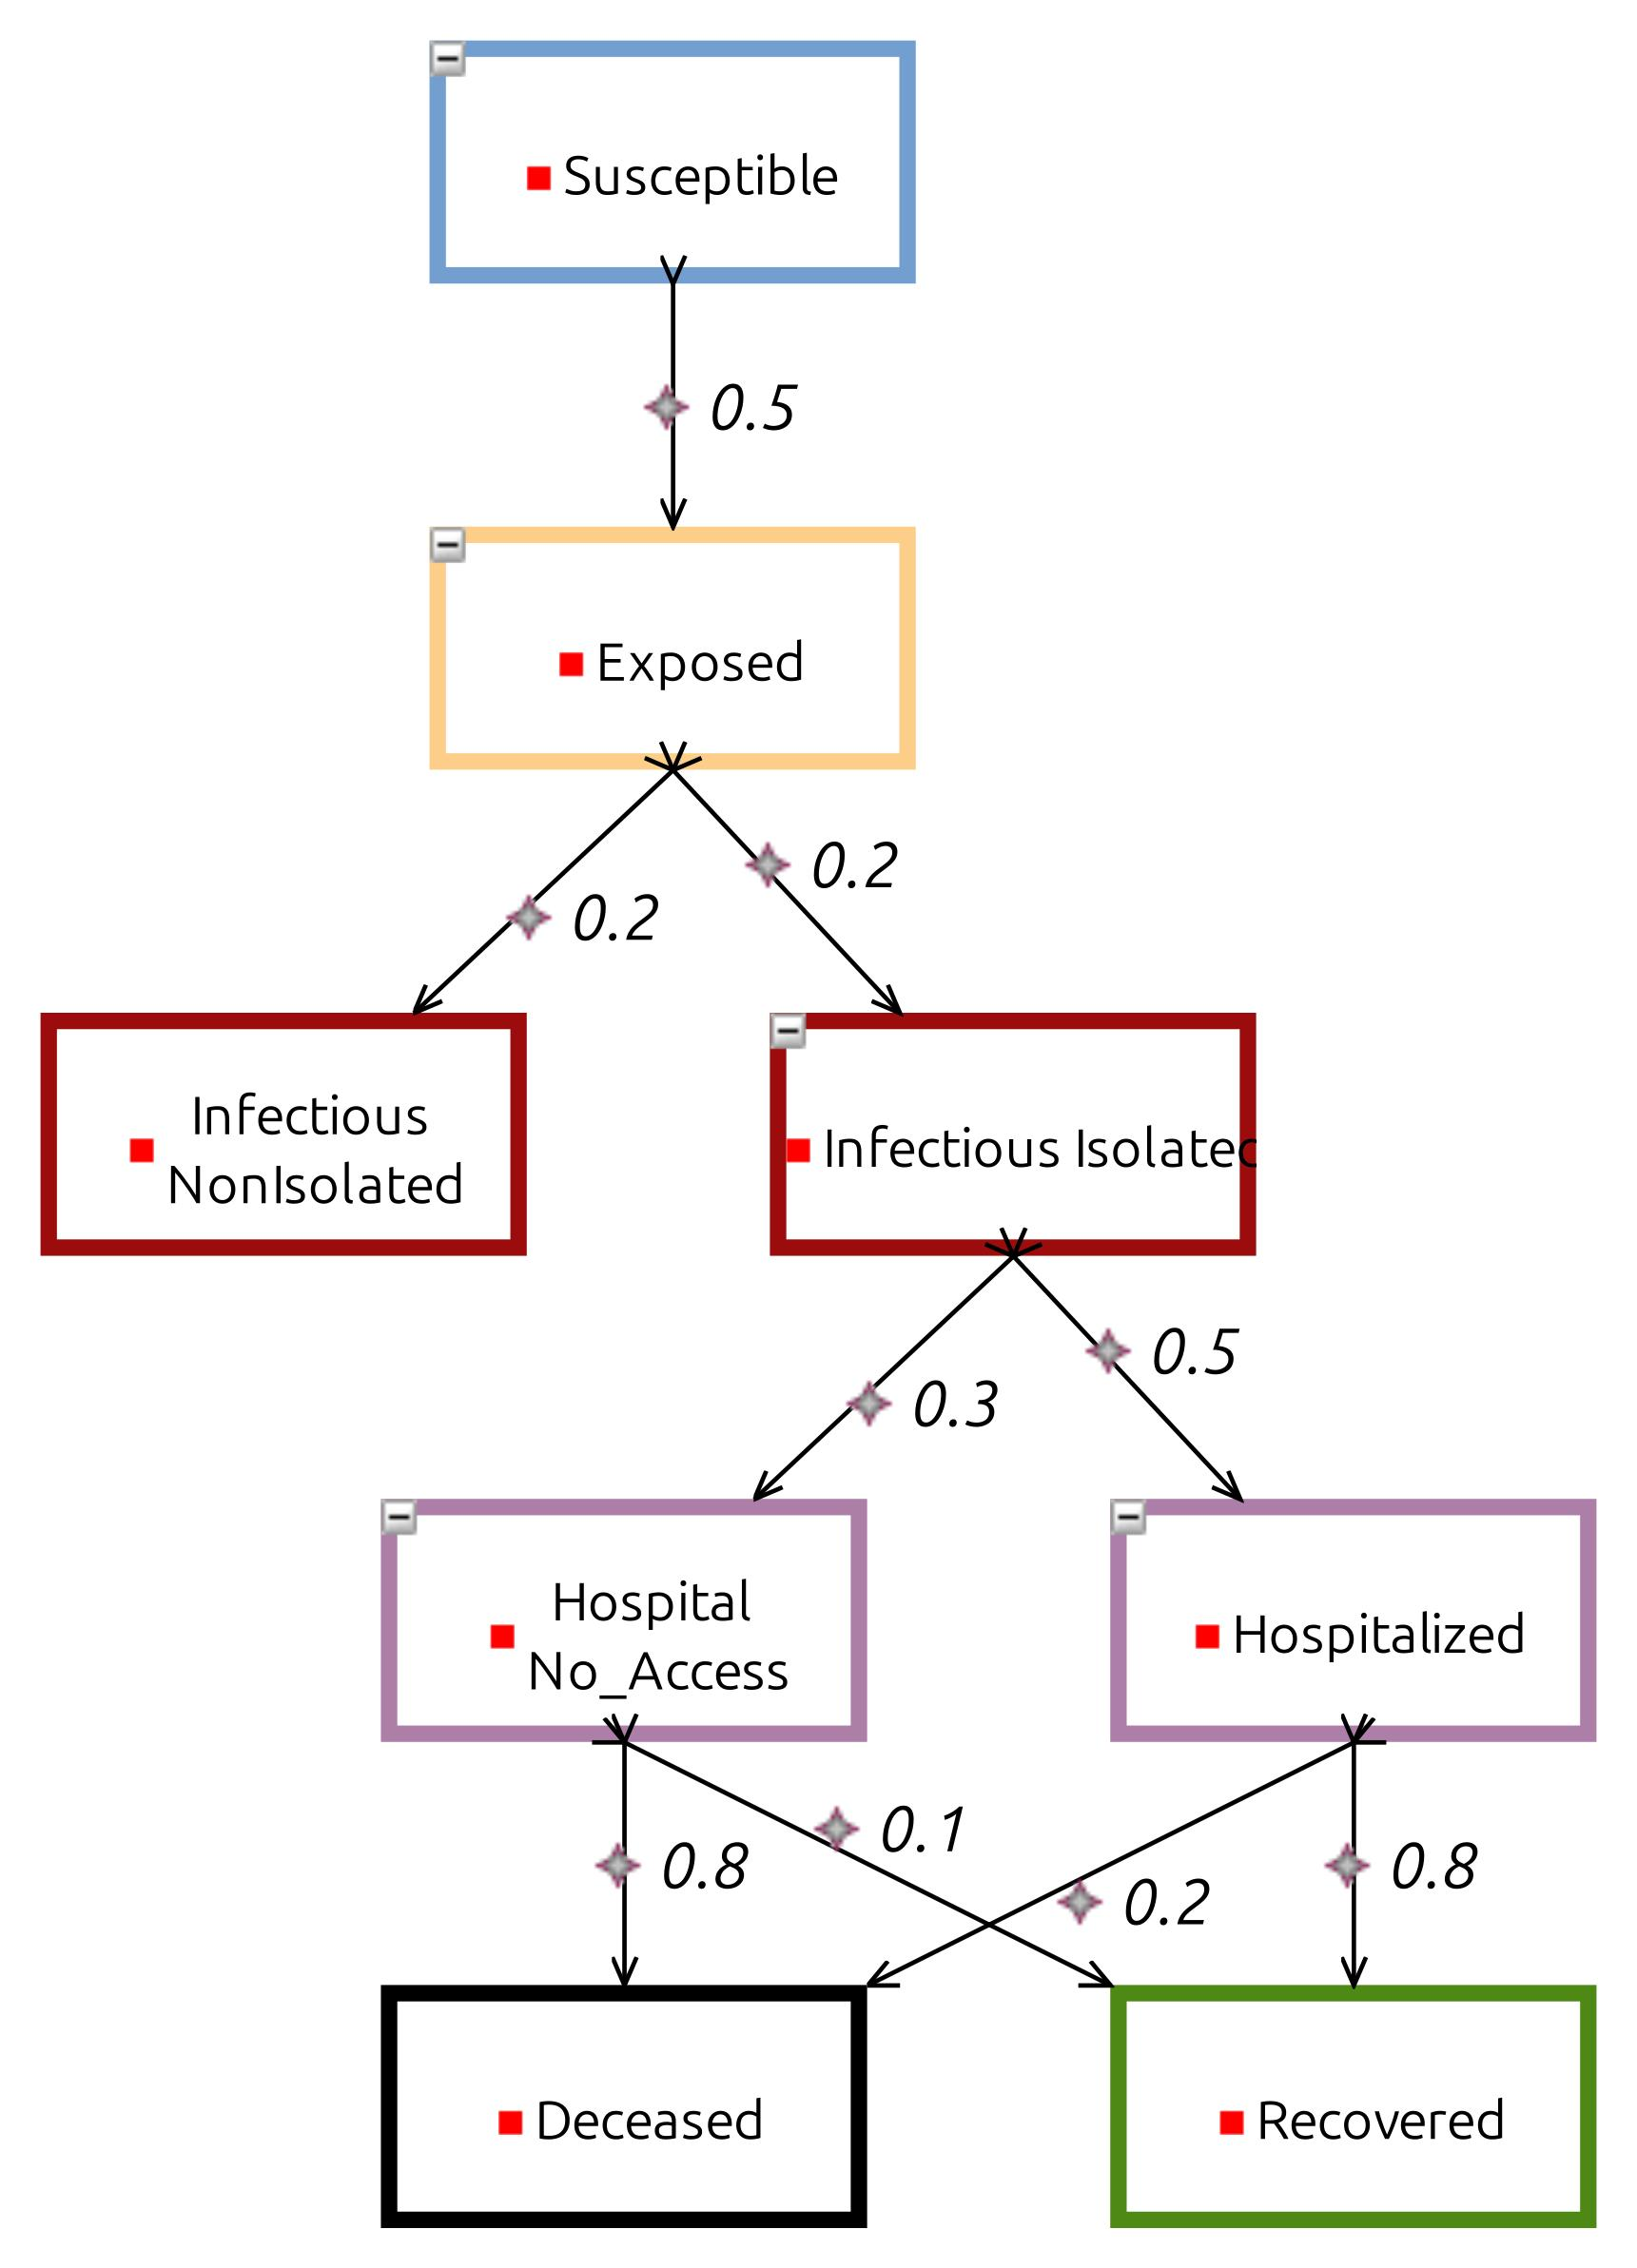
\includegraphics[width=\textwidth]{Figures/paper3.jpg}
  \caption{$m_3$}
  \label{fig:prototype_m3}
\end{subfigure}
\caption{Corpus of prior compartmental models to consult.
}
\label{fig:prototype_submodels}
\end{figure}

% \subsection{Approach}
%to help epidemiologists seamlessly reuse modeling ideas from previous models and rapidly integrate them into a prototype model, which they can use for further development. Below, we explain the four steps of our approach.

\subsubsection{Workflow}
\label{sec:prototyping_workflow}

We implemented the workflow as an external layer on top of EpiMDE. It operationalizes a prototyping-specific notion of ``relevance'' to support rapid model construction under time pressure. EpiMDE itself does not prescribe a canonical relevance metric or workflow; rather, it provides the model representations, APIs, and analysis hooks required to implement such workflows.

Concretely, the workflow layer leverages programmatic access to EpiMDE models and metamodel instances, stable element identifiers, and integration with third-party analysis tools. The heuristics used to identify and rank potentially relevant components are intentionally workflow-specific, and are presented here to demonstrate that EpiMDE provides sufficient expressive power and extensibility to support domain-specific modeling workflows.

We build the interactive rapid prototyping EpiMDE layer in four steps.

\paragraph{Variation Point Extraction:} 
First, we identify commonalities and differences in the input corpus.
For example, the compartment \textit{Susceptible} appears in all models ($m_1$-$m_3$), so we consider it a commonality indicating the same epidemiological concept. 
On the other hand, the compartment labeled \textit{Hospitalized} only appears in $m_3$: the other models do not concern themselves with this concept.

Note that although the models in the corpus may describe different diseases, identifying variation points remains meaningful. Many epidemiological concepts, such as the \textit{Susceptible} compartment, represent fundamental population states rather than disease-specific mechanisms. Thus, commonalities can still capture shared modeling structures that are valuable for constructing new prototypes even when the models target distinct pathogens. Of course, if the input corpus contains models of the same disease, the identified variation points are likely to be more disease-specific and semantically aligned.

To systematically identify \textit{variation points}, we assign unique identifiers (IDs) to the model elements, as follows: 
%A variation point represents a model element in a way that allows us to determine whether it is shared across models or distinct. The IDs are defined as follows:
%\begin{itemize}
    %\item 
(a) For compartments, the ID is simply the name of the compartment.
    %\item 
(b) For rates, flows, etc., the ID is a combination of the source compartment ID, target compartment ID, and the flow rate expression.
%\end{itemize}
%
When two elements share the same IDs, they are considered the same, but if their IDs are different, they are treated as variants. 
%This step helps identify common parts shared among models, laying the groundwork for extracting meaningful \textit{features} in the next steps.

% In the first step, our tool extracts the variation points from the existing models that Carol intends to reuse.
In Carol's case, for example
%an ID to each model element to identify which variation points are shared or unique across models. For compartments, we use the compartment name as the Variation Point ID. For example,
in model $m_1$, EpiMDE creates IDs for compartments such as \textit{Susceptible} and \textit{Vaccinated} %, and \textit{Exposed}.% are treated as distinct variation points. 
and IDs for flows such as %the ID is constructed by combining the source and target compartments as well as the flow rate. For instance, 
$Susceptible\_Vaccinated\_0.2$. 
%refers to a flow from \textit{Susceptible} to \textit{Vaccinated} with a rate of 0.2. 
% Using these IDs allows the tool to consistently detect and assign variation points to models. 
We show the complete list of variation points assigned to the models $m_1$, $m_2$, and $m_3$ in the Appendix Table~\ref{tab:prototype_variation_points}.


\paragraph{Feature Identification:} 
Next, we identify collections of variation points that appear together in the corpus and cluster them accordingly. 
These clusters likely represent features~\cite{berger2015feature}, pending confirmation by the epidemiologist.
We use Formal Concept Analysis (FCA), a mathematical framework used in data analysis and knowledge representation~\cite{ganter2012formal}
to classify objects based on shared attributes. 
Specifically, we integrated EpiMDE with FCA4J library~\cite{gutierrez2022fca4j}, 
which allows us to identify recurring patterns based on their shared variation points.%, identified by their unique IDs. 
%This allows us to detect shared variation points across different models, 
%that appear as recurring patterns that may represent modeling ideas or specific concepts that can be meaningfully reused together. 
%We then cluster these variation points to
We can thus identify potentially reusable components derived from existing models.
%
EpiMDE does this interactively, allowing Carol to change the automatically identified clusters.
This gives the epidemiologist the flexibility to split or reorganize clusters in case the mechanical clustering missed some relevant semantic nuance.
%This flexibility is important as some clusters might contain elements that are not related to each other, or the epidemiologist may prefer to reorganize them based on the specific needs of their study. 
We further prompt the epidemiologist to assign a meaningful label to each cluster. 
%These labels will make it easier for them to refer to and recognize the clusters further in the process. 
Once finalized and labeled, the refined clusters are henceforth referred to as \textit{features}. 


For Carol's three models
%In the second step, we apply Formal Concept Analysis (FCA) to the three models and their associated variation point IDs. 
FCA detects maximal groups of models that share a maximal set of variation points. 
We then cluster each of the identified sets of shared variation points to show the potential building blocks of existing models. 
For example, FCA identifies that all models share $Susceptible$, $Exposed$, and $Recovered$, which we put in the same cluster. 
% This set is identified by FCA, and we put them into the same cluster. 
This suggests that they often appear together and may represent a commonly reused pattern. 
Another example is the cluster formed by $Vaccinated$, $Susceptible\_Vaccinated\_0.2$, and $Vaccinated\_Susceptible\_0.3$, shared between $m_1$ and $m_2$. 
The fact that these co-occur in more than one place, indicates they might represent a common modeling idea that Carol would want to reuse together.

As a result of this step, EpiMDE generates the Appendix Table~\ref{tab:prototype_clusters}, which presents the clustered variation points. 
The table also includes a \textit{ClusterLabel} column initially left blank, allowing Carol to assign meaningful labels to each cluster. 
Carol can also refine and adapt the clusters as needed. 
We assume that she assigns the labels shown in the \textit{ClusterLabel} column and leaves the automatically identified clusters unchanged. 
Based on Carol's decision, each row in Table~\ref{tab:prototype_clusters} is considered to contain one \textit{feature}. 



\paragraph{Feature Relationship Identification:} Next, we identify relationships between features, such as dependency or mutual exclusivity. 
We always identify two relationships by default: 
%\begin{itemize}
    %\item 
(a)    A feature that contains a flow is always dependent on any other feature(s) containing the flow's source and target compartments. This ensures that compartments are well formed graphs.
    %This ensures that if we want to include the former in the prototype model, we also include the latter.
    %\item 
(b)    We assume that only one flow can exist between two compartments\footnote{Since compartmental models visualize differential equations, multiple arrows between the same compartments are redundant: they can be collapsed into a single arrow labeled with the sum of the rates. For our purposes, where the goal is to identify variation points between models, we treat differing rates as mutually exclusive alternatives, rather than cumulative effects.}. Thus if a feature contains a flow between two Compartments $A$ and $B$, it is mutually exclusive to  features that include other flows between $A$ and $B$.
%\end{itemize}
EpiMDE also prompts the epidemiologist to refine, customize and extend the set of identified feature relationships.
The resulting set of relationships are encoded in propositional logic, using the LogicNG library~\cite{logicng}.

In Carol's case, 
%In the next step, considering the features and the variation points each one contains, we identify the logical dependencies between features.
EpiMDE by default identifies the relatioship $Vaccination \Rightarrow Core\_SER$. 
This is because the $Vaccination$ feature includes a flow from \textit{Susceptible} to \textit{Vaccinated}. 
This flow relies on the existence of the $Susceptible$ compartment, which is part of the $Core\_SER$ feature, so $Vaccination$ depends on $Core\_SER$. 

Carol's case also includes mutual exclusivity relationships between features, such as the relationship
$Symptom\_Severity \Rightarrow \neg{Isolated\_Hospital} \land \neg{Exposed\_Isolation\_States}$. 
This is because $Symptom\_Severity$ has a flow from \textit{Susceptible} to \textit{Exposed} with a rate of 0.4, 
while $Isolated\_Hospital$ and $Exposed\_Isolation\_States$ also have flows between the same two compartments but with different rates. 
Based on our assumption that a compartmental model does not contain multiple flows between the same source and target compartments, 
EpiMDE identifies these features as mutually exclusive. 
The full set of the identified logical dependencies between features in Carol's example is available in the Zenodo replication package~\cite{zenodo_17806440}. 
In EpiMDE, Carol can further review, edit, or add to these constraints as needed. 




\paragraph{Feature Selection and Prototype Generation:} %With the features and necessary logical relationships between them at hand, it is time to construct the prototype model. 
To construct the prototype, Carol is prompted to select which combination of features she wants to include in her prototype.
%We ask the epidemiologist to select the features to include in their prototype model. 
%Providing a labeled list of features, using the labels that the epidemiologist assigned, makes it much easier for them to recognize and choose the relevant features that they want to include based on their specific modeling goals.
The epidemiologist can do this using the feature labels defined in Step 2.
%
To ensure her selection is valid with respect to the dependencies identified in Step 3, 
EpiMDE conjuncts all relevant relationship formulas and makes a satisfiability check using LogicNG. 
%the validity of user selection, we check its satisfiability according to the defined dependency rules, using an SAT solver along with the previously constructed LogicNG logical formulas. 
If the result is UNSAT, the epidemiologist is given a warning and asked to adapt her feature selection.
%If the solver finds the selection unsatisfiable, it means the combination of selected features does not work together logically. 
With a valid feature selection, we generate a prototype compartmental model that includes the appropriate features.
We implemented the feature merging in Java using the EpiMDE metamodel.

In Carol's case, EpiMDE prompts her to select from the list of features to include in the prototype model. 
We suppose that she selects $Mortality$ and $Exposed\_Isolation\_States$. 
EpiMDE checks for the satisfiability of the logical dependencies of her selection. 
They are satisfiable, and EpiMDE generates the model shown in Figure~\ref{fig:prototype_result_model}. 
In addition to Carol's selected features, the prototype model contains the feature $Core\_SER$, which Carol did not directly choose, but it is required based on the logical relationships between features. 
Carol can then treat this generated model as a prototype that reuses features from previous models.
She can then use it as the basis to develop a complete model according to her needs, without having to re-implement these features.
%completed, meaning that while it contains the desired features from existing work, Carol can evolve it further and add novel aspects specific to her study. 

% \end{enumerate}

 
\begin{figure}[t]
  \centering
  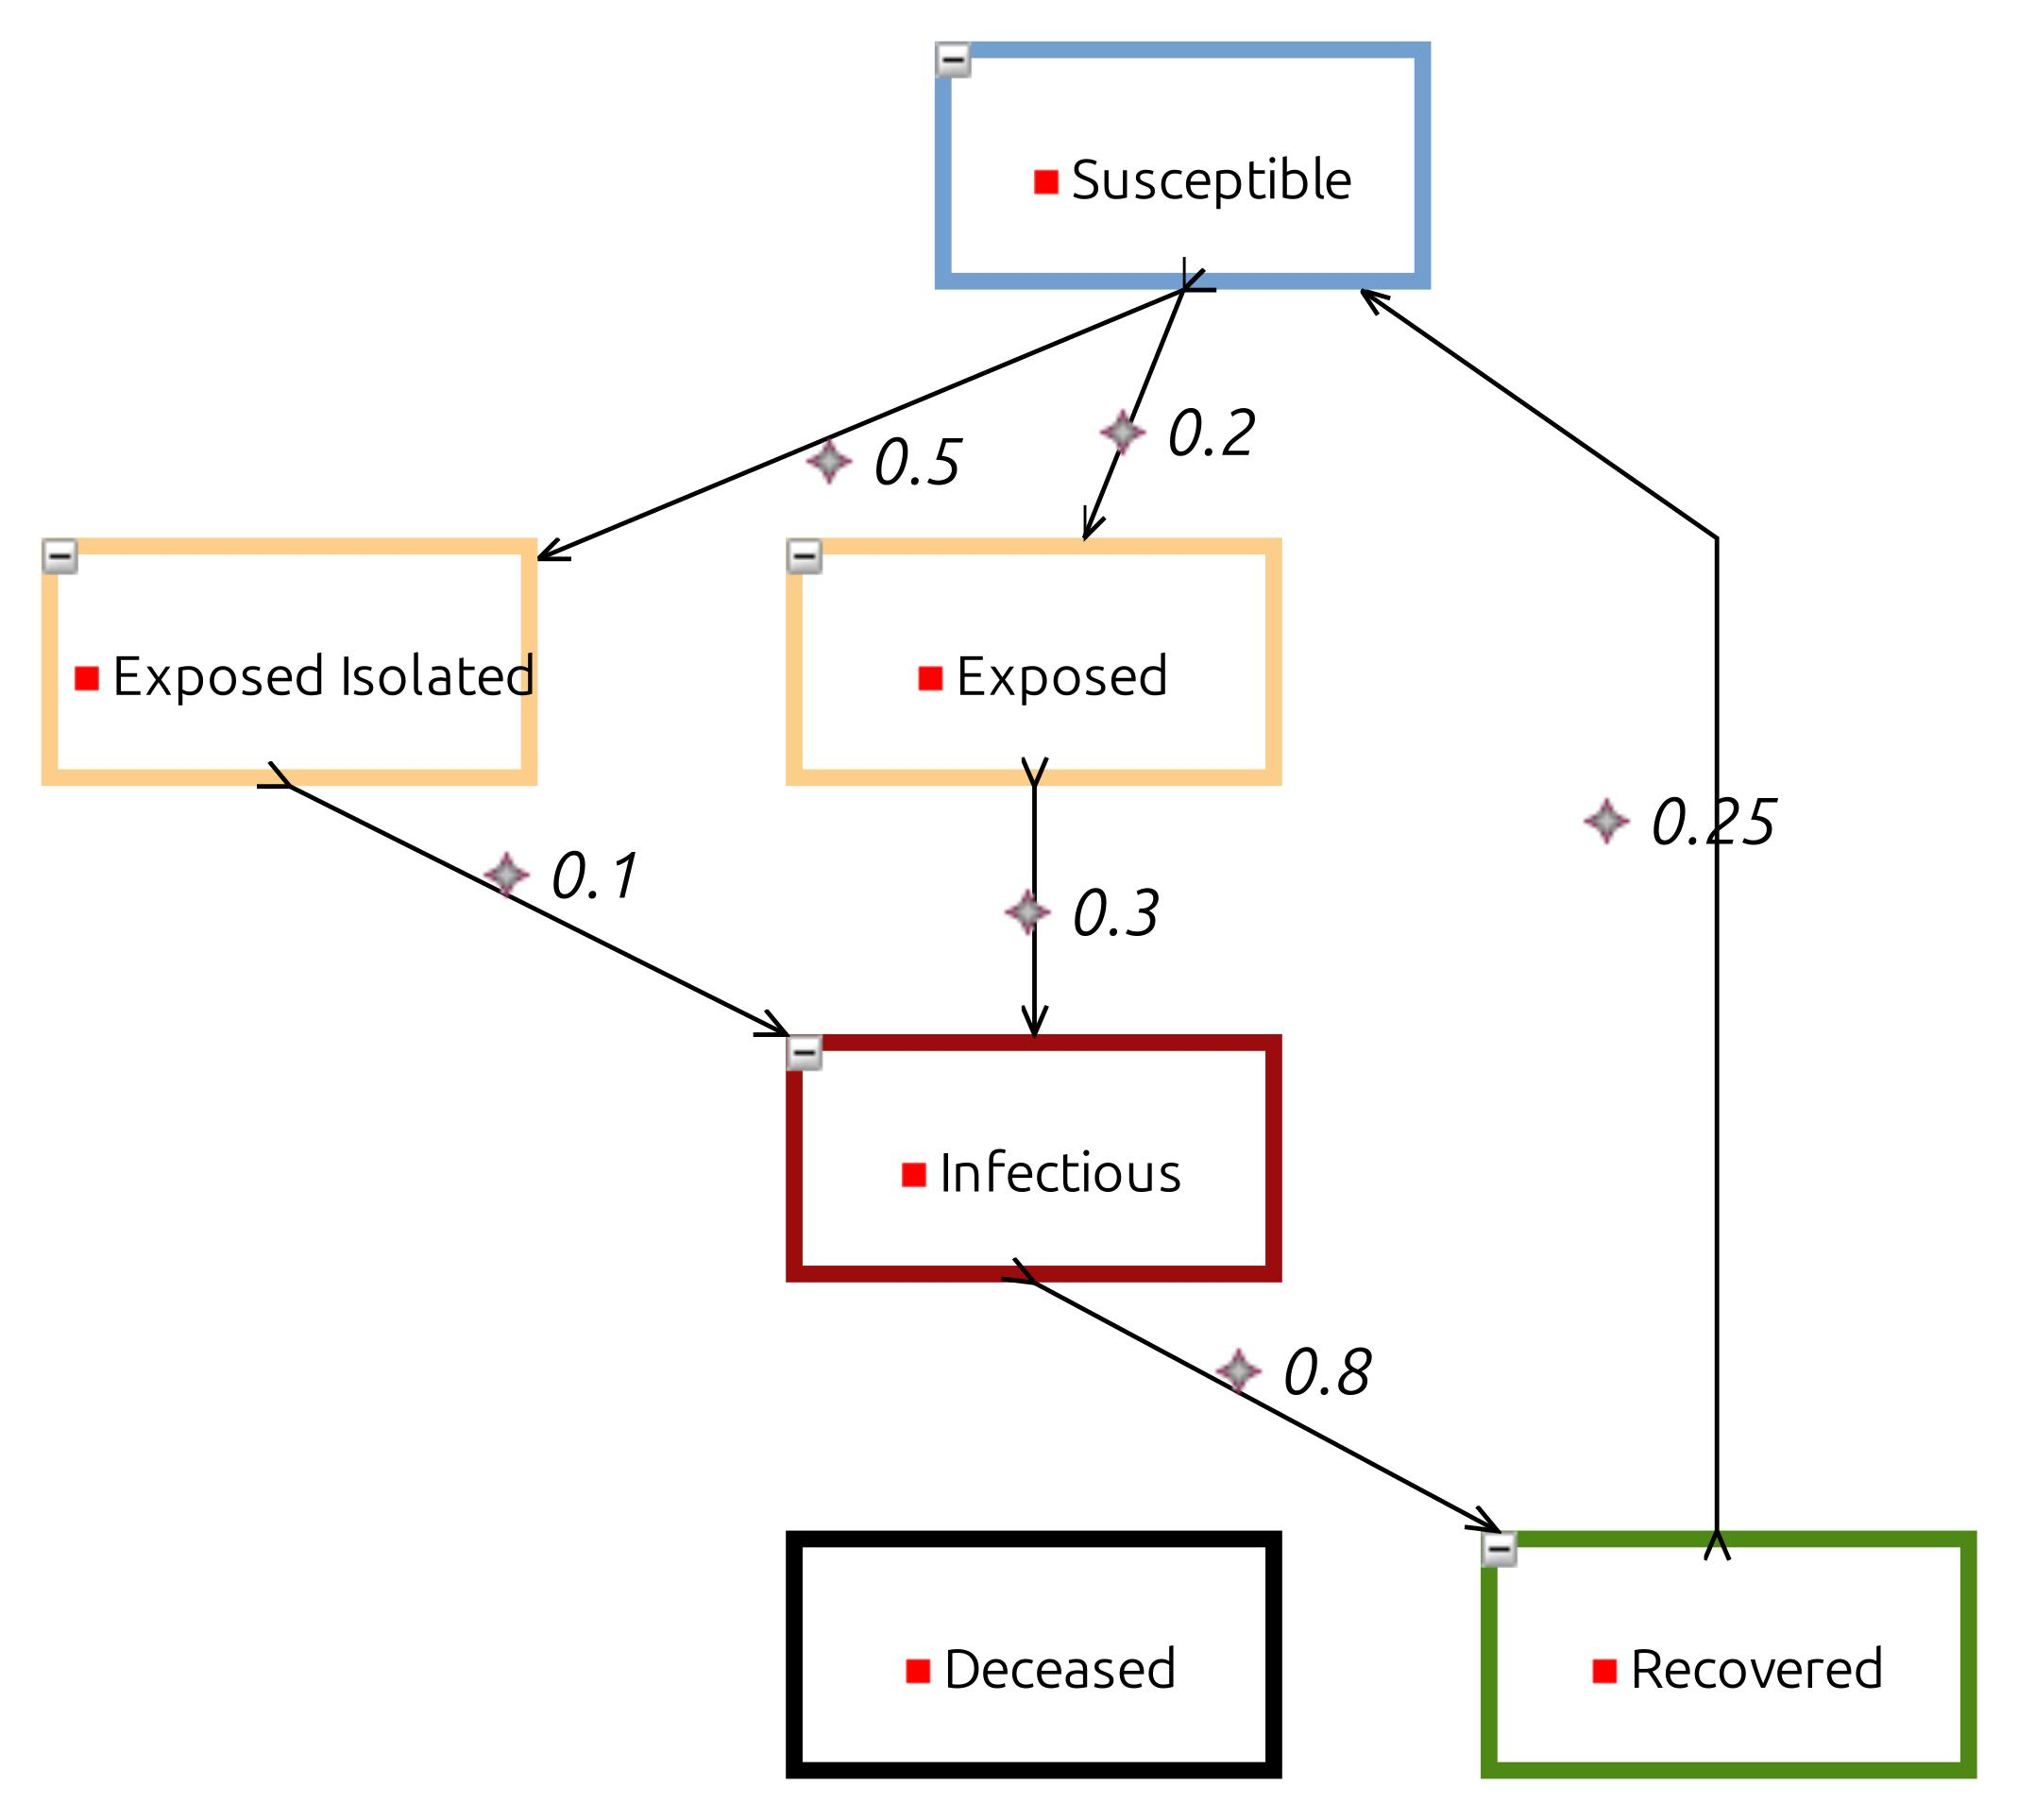
\includegraphics[width=0.5\textwidth]{Figures/fig9.jpg}
  \caption{The generated partially completed prototype model in EpiMDE containing Carol's selected features.}
  \label{fig:prototype_result_model}
\end{figure}

% \subsection{Discussion and Future Work}




